%  LaTeX support: latex@mdpi.com 
%  For support, please attach all files needed for compiling as well as the log file, and specify your operating system, LaTeX version, and LaTeX editor.

%=================================================================
%\documentclass[journal,article,submit,pdftex,moreauthors]{Definitions/mdpi}  
\documentclass[preprints,article,submit,pdftex,moreauthors]{Definitions/mdpi} 
% For posting an early version of this manuscript as a preprint, you may use "preprints" as the journal. Changing "submit" to "accept" before posting will remove line numbers.

\newtheoremstyle{axiomstyle}
  {}{}                 % razmaci
  {\itshape}           % telo
  {}                   % indent
  {\bfseries}          % naslov
  {.}                  % tačka iza broja
  {0.5em}              % razmak
  {\thmname{#1}~\thmnumber{#2}\thmnote{ (#3)}} % OVO PRIKAZUJE (RG0...)
  
\theoremstyle{axiomstyle}
\newtheorem{axiom}{Axiom}
%\newtheorem{remark}{Remark}[section]
%--------------------
% Class Options:
%--------------------
%----------
% journal
%----------
% Choose between the following MDPI journals:
% accountaudit, acoustics, actuators, addictions, adhesives, adolescents, aerobiology, aerospace, agriculture, agriengineering, agrochemicals, agronomy, ai, aichem, aieng, aimater, aimed, aipa, air, aisens, algorithms, allergies, alloys, amh, analog, analytica, analytics, anatomia, anesthres, animals, antibiotics, antibodies, antioxidants, applbiosci, appliedchem, appliedmath, appliedphys, applmech, applmicrobiol, applnano, applsci, aquacj, architecture, arm, arthropoda, asc, asi, astronautics, astronomy, atmosphere, atoms, audiolres, automation, axioms, bacteria, batteries, bdcc, beverages, biochem, bioengineering, biologics, biology, biomass, biomechanics, biomed, biomedicines, biomedinformatics, biomimetics, biomolecules, biophysica, bioresourbioprod, biosensors, biosphere, biotech, birds, blockchains, bloods, blsf, brainsci, breath, buildings, cancers, carbon, cardio, cardiogenetics, cardiovascmed, catalysts, cells, ceramics, challenges, chemengineering, chemistry, chemosensors, chemproc, children, chips, cimb, civileng, cleantechnol, climate, clinbioenerg, clinpract, clockssleep, cmd, cmtr, coasts, coatings, colloids, colorants, commodities, complexities, complications, compounds, computation, computers, condensedmatter, conservation, constrmater, cosmetics, covid, crops, cryo, cryptography, crystals, csmf, ctn, culture, curroncol, cyber, dairy, data, ddc, dentistry, dermato, dermatopathology, designs, devices, dhi, diabetology, diagnostics, dietetics, digital, disabilities, diseases, diversity, dna, drones, dynamics, earth, ebj, ecm, ecologies, edm, eesp, electricity, electrochem, electronicmat, electronics, encyclopedia, endocrines, energies, eng, engproc, entomology, entropy, environments, environremediat, epidemiologia, epigenomes, esa, est, fermentation, fibers, fintech, fire, fishes, fluids, foods, forecasting, forensicsci, forests, fossstud, foundations, fractalfract, fuels, future, futureinternet, futurepharmacol, futurephys, futuretransp, galaxies, gases, gastroent, gastrointestdisord, gastronomy, gels, genes, geographies, geohazards, geomatics, geometry, geosciences, geotechnics, geriatrics, germs, glacies, grasses, green, greenhealth, gucdd, hardware, hazardousmatters, healthcare, hearts, hemato, hematolrep, hep, heritage, higheredu, highthroughput, horticulturae, hospitals, hydrobiology, hydrogen, hydrology, hydropower, hygiene, idr, iic, ijem, ijerph, ijgi, ijmd, ijms, ijns, ijom, ijpb, ijt, ijtm, ijtpp, ime, immuno, informatics, information, infrastructures, inorganics, insects, instruments, inventions, iot, j, jaestheticmed, jal, jcdd, jcm, jcp, jcrm, jcs, jcto, jdad, jdb, jdream, jemr, jeta, jfb, jfmk, jgbg, jgg, jimaging, jlpea, jmahp, jmmp, jmms, jmp, jmse, jne, jnt, jof, joi, joitmc, joma, jop, joptm, jor, jox, jpbi, jphytomed, jpm, jsan, jtaer, jvd, jzbg, kidneydial, kinasesphosphatases, knowledge, labmed, laboratories, lae, land, life, lights, limnolrev, lipidology, liquids, livers, logics, logistics, lubricants, lymphatics, machines, macromol, magnetism, magnetochemistry, make, marinedrugs, materials, materproc, mathematics, mca, measurements, medicina, medicines, medsci, membranes, merits, metabolites, metals, meteorology, methane, metrics, metrology, micro, microarrays, microbiolres, microelectronics, micromachines, microorganisms, microplastics, microwave, minerals, mining, mmphys, modelling, molbank, molecules, mps, msf, mti, multimedia, muscles, nanoenergyadv, nanomanufacturing, nanomaterials, ncrna, ndt, network, neuroglia, neuroimaging, neurolint, neurosci, nitrogen, notspecified, nursrep, nutraceuticals, nutrients, obesities, occuphealth, oceans, ohbm, onco, optics, oral, organics, organoids, osteology, oxygen, pandemics, parasites, parasitologia, particles, pathogens, pathophysiology, pediatrrep, pets, pharmaceuticals, pharmaceutics, pharmacoepidemiology, pharmacy, philosophies, photochem, photonics, phycology, physchem, physics, physiologia, plants, plasma, platforms, pollutants, polymers, polysaccharides, populations, poultry, powders, precipitation, precisoncol, preprints, proceedings, processes, prosthesis, proteomes, psf, psychiatryint, psychoactives, purification, quantumrep, quaternary, qubs, radiation, rdt, reactions, realestate, receptors, recycling, regeneration, remotesensing, reports, reprodmed, resources, rheumato, rjpm, robotics, rsee, ruminants, safety, sci, scipharm, sclerosis, seeds, sensors, separations, sexes, shi, signals, sinusitis, siuj, skins, smartcities, sna, societies, software, soilsystems, solar, solids, spectroscj, sports, standards, stats, std, stratsediment, stresses, surfaces, surgeries, suschem, sustainability, symmetry, synbio, systems, tae, targets, taxonomy, technologies, telecom, test, textiles, thalassrep, therapeutics, thermo, timespace, tomography, toxics, toxins, tph, transplantology, transportation, traumacare, traumas, tri, tropicalmed, universe, urbansci, uro, vaccines, vehicles, venereology, vetsci, vibration, virtualworlds, viruses, vision, waste, water, welding, wem, wevj, wild, wind, women, world, zoonoticdis

%---------
% article
%---------
% The default type of manuscript is "article", but can be replaced by: 
% abstract, addendum, article, benchmark, book, bookreview, briefcommunication, briefreport, casereport, changes, clinicopathologicalchallenge, comment, commentary, communication, conceptpaper, conferenceproceedings, correction, conferencereport, creative, datadescriptor, discussion, entry, expressionofconcern, extendedabstract, editorial, essay, erratum, fieldguide, hypothesis, interestingimages, letter, meetingreport, monograph, newbookreceived, obituary, opinion, proceedingpaper, projectreport, reply, retraction, review, perspective, protocol, shortnote, studyprotocol, supfile, systematicreview, technicalnote, viewpoint, guidelines, registeredreport, tutorial,  giantsinurology, urologyaroundtheworld
% supfile = supplementary materials

%----------
% submit
%----------
% The class option "submit" will be changed to "accept" by the Editorial Office when the paper is accepted. This will only make changes to the frontpage (e.g., the logo of the journal will get visible), the headings, and the copyright information. Also, line numbering will be removed. Journal info and pagination for accepted papers will also be assigned by the Editorial Office.

%------------------
% moreauthors
%------------------
% If there is only one author the class option oneauthor should be used. Otherwise use the class option moreauthors.

%---------
% pdftex
%---------
% The option pdftex is for use with pdfLaTeX. Remove "pdftex" for (1) compiling with LaTeX & dvi2pdf (if eps figures are used) or for (2) compiling with XeLaTeX.

%=================================================================
% MDPI internal commands - do not modify
\firstpage{1} 
\makeatletter 
\setcounter{page}{\@firstpage} 
\makeatother
\pubvolume{1}
\issuenum{1}
\articlenumber{0}
\pubyear{2026}
\copyrightyear{2025}
%\externaleditor{Firstname Lastname} % More than 1 editor, please add `` and '' before the last editor name
\datereceived{ } 
\daterevised{ } % Comment out if no revised date
\dateaccepted{ } 
\datepublished{ } 
%\datecorrected{} % For corrected papers: "Corrected: XXX" date in the original paper.
%\dateretracted{} % For retracted papers: "Retracted: XXX" date in the original paper.
%\doinum{} % Used for some special journals, like molbank
%\pdfoutput=1 % Uncommented for upload to arXiv.org
%\CorrStatement{yes}  % For updates
%\longauthorlist{yes} % For many authors that exceed the left citation part
%\IsAssociation{yes} % For association journals

%=================================================================
% Add packages and commands here. The following packages are loaded in our class file: fontenc, inputenc, calc, indentfirst, fancyhdr, graphicx, epstopdf, lastpage, ifthen, float, amsmath, amssymb, lineno, setspace, enumitem, mathpazo, booktabs, titlesec, etoolbox, tabto, xcolor, colortbl, soul, multirow, microtype, tikz, totcount, changepage, attrib, upgreek, array, tabularx, pbox, ragged2e, tocloft, marginnote, marginfix, enotez, amsthm, natbib, hyperref, cleveref, scrextend, url, geometry, newfloat, caption, draftwatermark, seqsplit
% cleveref: load \crefname definitions after \begin{document}

% TikZ libraries for logical structure diagram
\usetikzlibrary{shapes,arrows,positioning,fit,backgrounds,calc}

% Fix fancyhdr warning
\setlength{\headheight}{17.38797pt}

%=================================================================
% Please use the following mathematics environments: Theorem, Lemma, Corollary, Proposition, Characterization, Property, Problem, Example, ExamplesandDefinitions, Hypothesis, Remark, Definition, Notation, Assumption
%% For proofs, please use the proof environment (the amsthm package is loaded by the MDPI class).

%=================================================================
% Full title of the paper (Capitalized)
\Title{Recognition Geometry}

% Author Orchid ID: enter ID or remove command

% Author Orchid ID: enter ID or remove command
\newcommand{\orcidauthorA}{0009-0001-8868-7497} % Add \orcidA{} behind the author's name
%\newcommand{\orcidauthorA}{https://orcid.org/0009-0001-8868-7497} % Add \orcidA{} behind the author's name
\newcommand{\orcidauthorB}{0000-0002-0318-1092} % Add \orcidB{} behind the author's name
\newcommand{\orcidauthorC}{0000-0001-7212-4713} % Add \orcidC{} behind the author's name



% Authors, for the paper (add full first names)
\Author{Jonathan Washburn$^{1}$\orcidA{}, Milan Zlatanovi\'c $^{2,*}$\orcidB{} and
        Elshad Allahyarov$^{1,3,4,5}$\orcidC{} }

%\longauthorlist{yes}

% MDPI internal command: Authors, for metadata in PDF
\AuthorNames{Jonathan Washburn, Milan Zlatanovi\'c and Elshad Allahyarov}

% Affiliations / Addresses (Add [1] after \address if there is only one affiliation.)
\address{%
$^{1}$ \quad Recognition Physics Institute Austin, Texas, USA; jon@recognitionphysics.org\\
$^{2}$ \quad Faculty of Science and Mathematics, University of Ni\v s,  Serbia; zlatmilan@yahoo.com\\
$^{1}$ \quad Recognition Physics Institute, Austin, TX, USA;  \\
$^{3}$ \quad Institut für Theoretische Physik II: Weiche Materie, Heinrich-Heine-Universität Düsseldorf, Germany; \\ 
$^{4}$ \quad Theoretical Department, Joint Institute for High Temperatures, RAS, Moscow, Russia; \\  
$^{5}$ \quad Department of Physics, Case Western Reserve University, Cleveland, OH, USA; elshad.allakhyarov@case.edu}

% Contact information of the corresponding author
\corres{Correspondence: zlatmilan@yahoo.com}

% Current address and/or shared authorship
%\firstnote{Current address: Affiliation.}  
% Current address should not be the same as any items in the Affiliation section.

%\secondnote{These authors contributed equally to this work.}
% The commands \thirdnote{} till \eighthnote{} are available for further notes.

%\simplesumm{} % Simple summary

%\conference{} % An extended version of a conference paper

% Abstract (Do not insert blank lines, i.e. \\) 
\abstract{ We introduce Recognition Geometry (RG), an axiomatic framework in which
geometric structure is not assumed a priori, but it is derived.
The starting point of the theory is a configuration space together with
recognizers that map configurations to observable events.
Observational indistinguishability induces an equivalence relation,
and the observable space is obtained as a recognition quotient.
Locality is introduced through a neighborhood system, without assuming
any metric or topological structure.
A finite local resolution Axiom \ref{axiom:rg4} (RG3) formalizes the fact that any observer can
distinguish only finitely many outcomes in a local region. {\color{blue}We prove that the induced observable map \texorpdfstring{$\overline{R}:\mathcal{C}_R \to \mathcal{E}$}{R-bar: C\_R to E} is injective, establishing that observable states are uniquely determined by measurement outcomes with no hidden structure.}  %% \textcolor{blue}{[Response to Reviewer 1, Comment 1: Making key result explicit]}
{\color{blue}The framework connects deeply with existing approaches: \texorpdfstring{C\textsuperscript{*}}{C*}-algebraic quantum theory, information geometry, categorical physics, causal set theory, noncommutative geometry, and topos-theoretic foundations all share the measurement-first philosophy, yet RG provides a unified axiomatic foundation synthesizing these perspectives.}  %% \textcolor{blue}{[Response to Reviewer 1, Comments 1 \& 2: Positioning and related work]}
Comparative recognizers allow us to define order-type
relations based on operational comparison.
Under additional assumptions, quantitative notions of distinguishability
can be introduced in the form of recognition distances, defined as
pseudometrics. 
Several examples are provided, including threshold recognizers on
\texorpdfstring{$\mathbb{R}^n$}{R\^{}n}, discrete lattice models, quantum spin measurements, and an
example motivated by Recognition Science.
In the last part, we develop the composition of recognizers, proving that composite recognizers refine quotient structures and increase distinguishing power. We introduce symmetries and gauge equivalence, showing that gauge-equivalent configurations are necessarily observationally indistinguishable, though the converse does not hold in general.
A significant part of the axiomatic  framework  and the main constructions have been formalized in the Lean~4 proof assistant, providing an independent verification of logical consistency.}

% Keywords
\keyword{Recognition geometry, configuration spaces, event spaces, recognizer, quotient spaces,  resolution cells,  recognition distances} 

% The fields PACS, MSC, and JEL may be left empty or commented out if not applicable
%\PACS{J0101}
\MSC{51A05, 54A05, 03B30, 81P15, 18B99}
%\JEL{}

%%%%%%%%%%%%%%%%%%%%%%%%%%%%%%%%%%%%%%%%%%
% Only for the journal Diversity
%\LSID{\url{http://}}

%%%%%%%%%%%%%%%%%%%%%%%%%%%%%%%%%%%%%%%%%%
% Only for the journal Applied Sciences
%\featuredapplication{Authors are encouraged to provide a concise description of the specific application or a potential application of the work. This section is not mandatory.}
%%%%%%%%%%%%%%%%%%%%%%%%%%%%%%%%%%%%%%%%%%

%%%%%%%%%%%%%%%%%%%%%%%%%%%%%%%%%%%%%%%%%%
% Only for the journal Data
%\dataset{DOI number or link to the deposited data set if the data set is published separately. If the data set shall be published as a supplement to this paper, this field will be filled by the journal editors. In this case, please submit the data set as a supplement.}
%\datasetlicense{License under which the data set is made available (CC0, CC-BY, CC-BY-SA, CC-BY-NC, etc.)}

%%%%%%%%%%%%%%%%%%%%%%%%%%%%%%%%%%%%%%%%%%
% Only for the journal BioTech, Fishes, Neuroimaging and Toxins
%\keycontribution{The breakthroughs or highlights of the manuscript. Authors can write one or two sentences to describe the most important part of the paper.}

%%%%%%%%%%%%%%%%%%%%%%%%%%%%%%%%%%%%%%%%%%
% Only for the journal Encyclopedia
%\encyclopediadef{For entry manuscripts only: please provide a brief overview of the entry title instead of an abstract.}

%%%%%%%%%%%%%%%%%%%%%%%%%%%%%%%%%%%%%%%%%%
% Different journals have different requirements. Please check the specific journal guidelines in the "Instructions for Authors" on the journal's official website.
%\addhighlights{yes}
%\renewcommand{\addhighlights}{%
%
%\noindent The goal is to increase the discoverability and readability of the article via search engines and other scholars. Highlights should not be a copy of the abstract, but a simple text allowing the reader to quickly and simplified find out what the article is about and what can be cited from it. Each of these parts should be devoted up to 2~bullet points.\vspace{3pt}\\
%\textbf{What are the main findings?}
% \begin{itemize}[labelsep=2.5mm,topsep=-3pt]
% \item First bullet.
% \item Second bullet.
% \end{itemize}\vspace{3pt}
%\textbf{What are the implications of the main findings?}
% \begin{itemize}[labelsep=2.5mm,topsep=-3pt]
% \item First bullet.
% \item Second bullet.
% \end{itemize}
%}



%%%%%%%%%%%%%%%%%%%%%%%%%%%%%%%%%%%%%%%%%%
\begin{document}

%% REVISION NOTE: Changes made in response to Reviewer 1's comments are highlighted in \textcolor{blue}{blue} 
%% and annotated with comment numbers [Comment 1-4] throughout the document.

%%%%%%%%%%%%%%%%%%%%%%%%%%%%%%%%%%%%%%%%%%
 


\newcommand{\config}{\mathcal{C}}
\newcommand{\configR}{\mathcal{C}_R}

\section{Motivation and Introduction}

\subsection{\texorpdfstring{\textcolor{blue}{The Classical Paradigm}}{The Classical Paradigm}}  %% \textcolor{blue}{[Response to Reviewer 1, Comments 1 \& 2: Explicit conceptual background]}

In geometry, from Euclid's space to Riemann's manifolds, the usual approach is to begin with a set of points equipped with some structure.
Objects (points, lines, planes, etc.) are then located in the space, and one studies how they interact and what can be measured. Measurement is usually modeled as a function assigning an observable value
to a pre-existing state, usually written in the form \(f(x) \in \mathbb{R}.
\)
In this classical viewpoint, the existence of the state $x$ is taken to be
ontologically prior to the measurement $f(x)$.  This space-first paradigm has dominated geometric thinking for over two millennia and remains 
the foundation of modern mathematical physics.


In the formulation of mathematical physics, one begins with a space or a spacetime manifold $M$, equipped with a topology $T$, a
differential structure $A$, and sometimes a metric tensor $g$.
Observables and measurements are then defined as functions on this space. While most of these points are not directly
observable, the use of a topology and a metric provides a precise
and flexible language for expressing locality, smoothness, and distance, which
has proven extremely effective in physical modeling. In this sense, the continuum
should be understood primarily as a mathematical idealization rather than as an ontological claim. Experimental limitations are typically incorporated
later, either through approximations or effective descriptions, without denying
the practical success of the underlying continuous framework.

This way of thinking dates back to Euclidean geometry, where the foundation was established through axioms regarding points, lines, and planes. Later, with Descartes, geometry became identified with $\mathbb{R}^n$, giving a coordinate‑based algebraic formulation. In the 19th century, non‑Euclidean ideas appeared in the work of Gauss, Lobachevsky, and Bolyai \cite{Zlat}. They still relied on the same foundation except for the fifth Euclidean postulate. This concept further evolved into the manifold framework \cite{Lee} used in General Relativity \cite{Einstein1916,Wald}, where space-time is modeled as a smooth 4‑dimensional continuum \cite{Penrose,Weyl}. {\color{blue}The geometric foundations of spacetime have been extensively analyzed from both physical \cite{Malament,Geroch} and philosophical perspectives \cite{Ellis}.} Even in Quantum Mechanics, the underlying Hilbert space is again a continuous structure built over the field of complex numbers \cite{Riesz}. {\color{blue}The mathematical formulation of quantum theory through operator algebras \cite{Gelfand} and functional analysis \cite{Segal} further reinforced the continuous paradigm.} In this sense, the assumption of a pre‑existing continuous substrate appears almost everywhere in modern theoretical physics.

\subsection{\texorpdfstring{\textcolor{blue}{Operational and Measurement-Based Approaches}}{Operational and Measurement-Based Approaches}}  %% \textcolor{blue}{[Response to Reviewer 1, Comments 1 \& 2: Explicit positioning]}

Despite this classical picture, the operational foundations of quantum theory have long emphasized the primacy of measurement over state. Von Neumann's axiomatization of quantum mechanics \cite{vonNeumann} placed measurement postulates on equal footing with unitary evolution, while the Wheeler-Zurek anthology \cite{WheelerZurek} documented decades of debate over whether quantum states exist independently of observation. More recently, operational approaches \cite{Hardy,Piron} and quantum Bayesian (QBist) interpretations \cite{Fuchs,Caves} have argued that quantum theory is fundamentally a calculus of expectations about measurement outcomes, not a description of an observer-independent reality. {\color{blue}The relational interpretation of quantum mechanics \cite{RQM,Laudisa} further suggests that quantum states are not absolute but relative to observers, reinforcing the measurement-centric viewpoint. Foundational investigations \cite{Isham,Landsman,Varadarajan} have explored the mathematical structures underlying quantum theory, while quantum logic approaches \cite{Svozil,Piron} reformulate the theory in terms of lattices of propositions rather than points in Hilbert space. Information-theoretic reformulations \cite{Zeilinger,Wigner} suggest that quantum mechanics may be fundamentally about information and distinguishability rather than ontological states in physical space.} 

In mathematical physics, the C*-algebraic formulation \cite{Bratteli,Haag} constructs quantum observables without presupposing a Hilbert space, instead deriving the space from the algebra of measurements. {\color{blue}The axiomatic foundations of quantum field theory \cite{Streater,Schweber} and the algebraic approach to quantum statistical mechanics \cite{Raimondi} further develop this operator-algebraic viewpoint. Convex-geometric methods \cite{Krein} provide structural results on state spaces and observables.} Category-theoretic approaches \cite{Abramsky,Coecke,Lawvere} similarly privilege processes (morphisms) over states (objects), emphasizing the relational structure of physical theories. {\color{blue}Higher categorical structures \cite{Lurie} and topos-theoretic foundations \cite{Topos} provide even more abstract frameworks for physical theories.} Information-geometric methods \cite{Jaynes,Amari1985,Amari2016} treat probability distributions as the fundamental objects, with the manifold structure emerging from distinguishability measures between distributions. {\color{blue}Fisher information metrics \cite{Frieden,Caticha} provide operational distance structures on statistical manifolds, showing how geometric properties arise from measurement precision. Bayesian and entropic approaches \cite{Kolmogorov,Suppes} further emphasize the primacy of operational inference over ontological commitment to space.}

In topology, the point-free approach via locales \cite{Johnstone,Vickers} and the categorical treatment of quotient spaces \cite{Adamek} demonstrate that spatial structure can be recovered from purely relational or logical primitives. {\color{blue}Formal topology \cite{Sambin} and categorical frameworks \cite{Ehresmann,Grothendieck} construct topological spaces from lattices of observable properties without presupposing an underlying set of points.}

{\color{blue}In quantum gravity and discrete approaches to spacetime, similar themes emerge. Causal set theory \cite{Bombelli,Sorkin} constructs spacetime from discrete causal relations, while loop quantum gravity \cite{LQG} derives geometric operators from gauge-theoretic foundations. Noncommutative geometry \cite{NCG} replaces point-sets with operator algebras. Computational approaches \cite{Wolfram} model physics through discrete rewriting rules. Information-theoretic proposals \cite{Verlinde} suggest that gravity and geometry emerge from entropy and information. Even foundational investigations of infinity and continuum \cite{Heller} question whether continuous structures are fundamental or emergent. Interpretive approaches to quantum field theory \cite{Teller} and structural realism \cite{Peirce} further emphasize relational over substantival foundations.}

These diverse threads suggest a common theme: \emph{the geometric structure of physical theory may be derivative rather than fundamental.} {\color{blue}Yet despite these hints, a systematic axiomatic framework that takes recognition (measurement) as primitive and derives space as a quotient structure has not been fully developed. Recognition Geometry fills this gap.}

These diverse threads suggest a common theme: \emph{the geometric structure of physical theory may be derivative rather than fundamental.} {\color{blue}Yet despite these hints, a systematic axiomatic framework that takes recognition (measurement) as primitive and derives space as a quotient structure has not been fully developed. Recognition Geometry fills this gap.}  %% \textcolor{blue}{[Response to Reviewer 1, Comment 1: Positioning RG]}

\subsection{\texorpdfstring{\textcolor{blue}{Related Work and Positioning}}{Related Work and Positioning}}  %% \textcolor{blue}{[Response to Reviewer 1, Comments 1 \& 2: Explicit positioning]}

{\color{blue}  %% [Response to Reviewer 1, Comments 1 \& 2: Detailed positioning]
While each of the approaches mentioned shares aspects of a measurement-first philosophy, none provides a minimal axiom system that derives observable space as a quotient from recognition maps. RG fills this gap by synthesizing operational, categorical, and information-theoretic ideas into a unified framework.

Recognition Geometry is intentionally positioned at the intersection of several measurement-first programs, but differs from each in its \emph{axiomatic target} and its \emph{construction principle}:
\begin{itemize}
\item \textbf{QBism / operational quantum foundations:} These approaches emphasize that quantum theory is about agents' expectations for measurement outcomes. RG abstracts this stance into a general mathematical framework where \emph{recognizers} are primitive and \emph{observable space} is derived as a quotient.
\item \textbf{Information geometry:} Information geometry equips statistical models with metrics derived from distinguishability. RG is more basic: it starts from recognition events and only later introduces order/distance via comparative recognizers, without presupposing probabilistic structure.
\item \textbf{Causal sets / discrete spacetime:} Discrete spacetime approaches postulate a discrete substrate. RG does not postulate discreteness; instead, discreteness can \emph{emerge operationally} from finite local resolution (RG3).
\item \textbf{Noncommutative geometry:} NCG replaces point-sets with operator algebras to encode geometry. RG is compatible with algebraic formulations but differs in emphasis: recognizers (maps to events) are primary, and quotienting by indistinguishability is the canonical construction of observable space.
\item \textbf{Topos approaches:} Topos-theoretic foundations reformulate physical theories in a new logical setting. RG retains classical logic/set theory but imports a similar methodological idea: reconstruct structure from operational/logical primitives rather than assuming a background manifold.
\end{itemize}
\noindent\textbf{What RG adds:} a minimal axiom system (RG0--RG4) for recognition-first models, a canonical quotient construction for observable space, a finite-resolution axiom (RG3) that encodes operational limitations, and comparative recognizers (RG4) as a route toward emergent order and distance.
}

\subsection{\texorpdfstring{\textcolor{blue}{Structure of the Paper}}{Structure of the Paper}}  %% \textcolor{blue}{[Response to Reviewer 1, Comment 1: Improved organization]}

The paper is structured as follows.
In \S\,2 we develop the axiomatic foundations of Recognition Geometry.
We introduce the primitive notion of a configuration space equipped with a
locality structure (\S\,2.1) and define recognizers as nontrivial maps to event
spaces (\S\,2.3).
The indistinguishability relation is defined in \S\,2.4, which leads to the
construction of resolution cells and the recognition quotient
(\S\,2.5--\S\,2.7). Theorem~\ref{thm:observable-injective},
shows that the induced observable map
$\overline{R}:\mathcal{C}_R\to\mathcal{E}$ is injective, meaning that distinct
observable states produce distinct events, and no hidden structure remains in
the quotient. We give several examples following the concept: threshold recognizers,
discrete lattices, quantum spin systems, and an instantiation from
Recognition Science, which illustrate the abstract constructions.
In \S\,3 we develop more advanced structures.
We introduce the composition of recognizers, finite local resolution,
and comparative recognizers.
We also show how order-type relations arise from comparative recognition
and how recognition distances can be constructed under additional
assumptions.
 

The main idea of Recognition Geometry (RG): a fundamental inversion of the usual viewpoint, where recognition is taken as primitive, and space with its geometric structure is derived from it.  

{\color{blue}\subsection{Logical Structure of the Framework}}  %% \textcolor{blue}{[Added from RG-Axioms-ver-11: Section 1.6]}

{\color{blue}Figure~\ref{fig:rg-structure} presents the logical architecture of Recognition Geometry, showing how the five axioms (RG0--RG4) lead to key definitions, which in turn yield the fundamental theorems establishing the framework's mathematical properties. The diagram illustrates the dependency chain: primitive axioms define recognizers, which induce indistinguishability relations, which generate recognition quotients, culminating in the major structural results.}

{\color{blue}
\smallskip
\noindent\textbf{Result hierarchy (reader's guide).} To clarify the logical and conceptual structure, we organize results into a ladder:
\begin{itemize}
\item \textbf{Foundational constructions (routine):} definitions and propositions establishing induced maps, quotient sets, and (when locality is given) induced topologies.
\item \textbf{Core structural theorems:} the injectivity of the induced observable map (Theorem~\ref{thm:observable-injective}) and the universal property of the recognition quotient (Theorem~\ref{thm:universal}), which show that $\mathcal{C}_R$ captures exactly the observable content of $R$.
\item \textbf{RG-distinctive consequences:} the role of finite local resolution (RG3) and comparative recognizers (RG4) in producing resolution cells, order-type relations, and operational notions of distance.
\end{itemize}
}

\begin{figure}[ht]
\centering
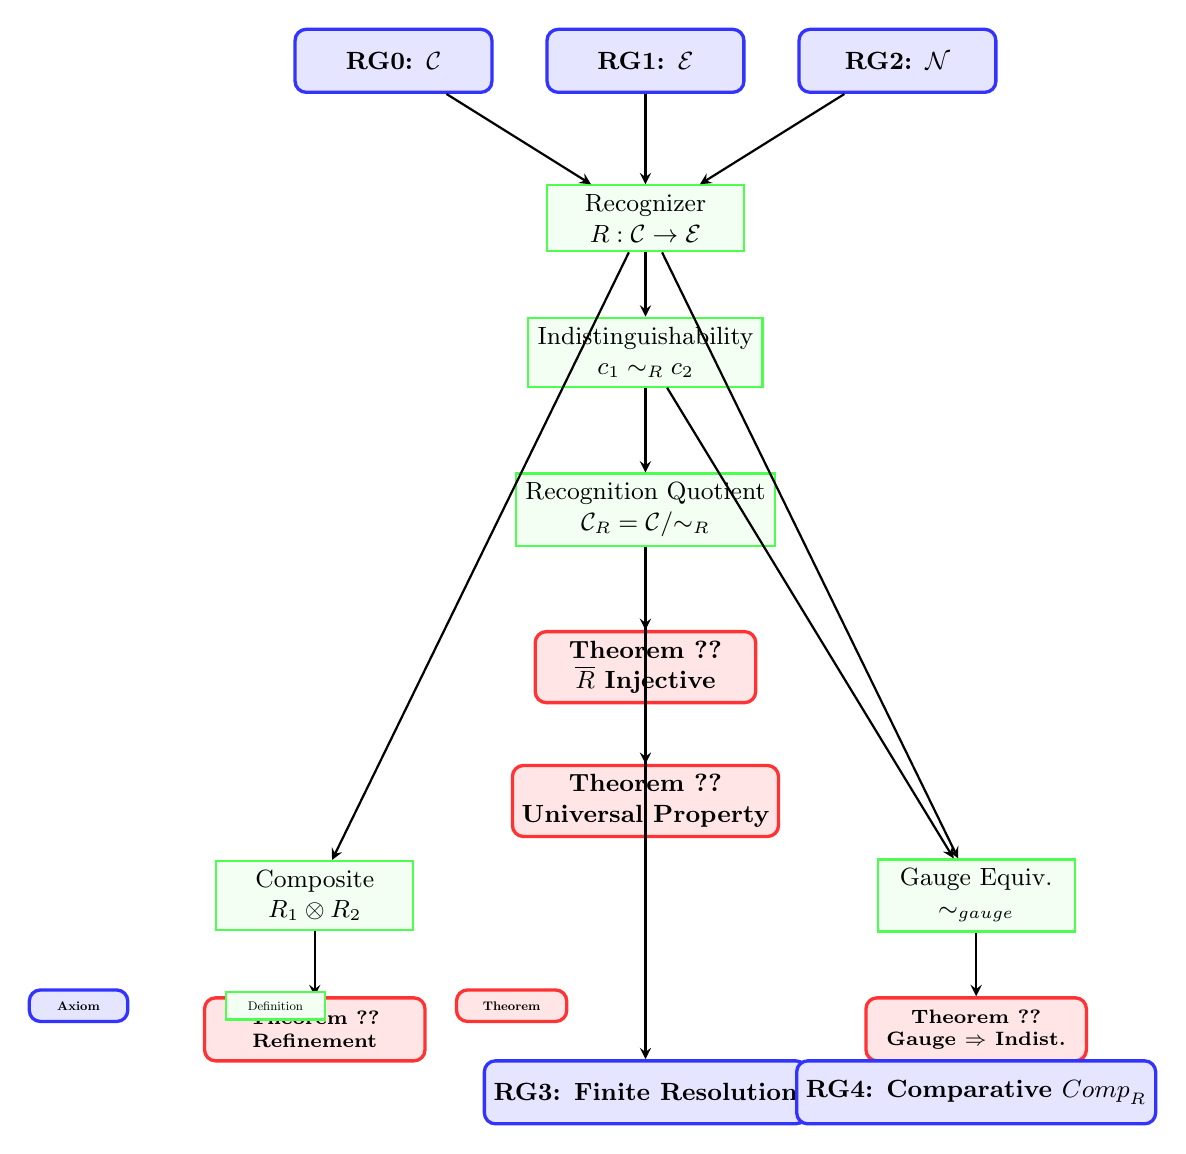
\begin{tikzpicture}[
    node distance=1.2cm, 
    auto,
    axiom/.style={rectangle, rounded corners, minimum width=2.5cm, minimum height=0.8cm, 
                  text centered, align=center, draw=blue!80, fill=blue!10, very thick, font=\small\bfseries},
    definition/.style={rectangle, minimum width=2.5cm, minimum height=0.7cm, 
                      text centered, align=center, draw=green!70, fill=green!5, thick, font=\small},
    theorem/.style={rectangle, rounded corners, minimum width=2.8cm, minimum height=0.8cm, 
                    text centered, align=center, draw=red!80, fill=red!10, very thick, font=\small\bfseries},
    arrow/.style={thick,->,>=stealth}
]

% Layer 0: Axioms
\node (RG0) [axiom] {RG0: $\mathcal{C}$};
\node (RG1) [axiom, right of=RG0, xshift=2cm] {RG1: $\mathcal{E}$};
\node (RG2) [axiom, right of=RG1, xshift=2cm] {RG2: $\mathcal{N}$};

% Layer 1: Basic Definitions
\node (recognizer) [definition, below of=RG1, yshift=-0.8cm] {Recognizer\\$R: \mathcal{C} \to \mathcal{E}$};
\node (indist) [definition, below of=recognizer, yshift=-0.5cm] {Indistinguishability\\$c_1 \sim_R c_2$};

% Layer 2: Quotient
\node (quotient) [definition, below of=indist, yshift=-0.8cm] {Recognition Quotient\\$\mathcal{C}_R = \mathcal{C}/{\sim_R}$};

% Major Theorems
\node (thm21) [theorem, below of=quotient, yshift=-0.8cm] {Theorem~\ref{thm:observable-injective}\\$\overline{R}$ Injective};
\node (thm22) [theorem, below of=thm21, yshift=-0.5cm] {Theorem~\ref{thm:universal}\\Universal Property};

% Advanced Structures
\node (composite) [definition, left of=thm22, xshift=-3cm, yshift=-1.2cm] {Composite\\$R_1 \otimes R_2$};
\node (thm31) [theorem, below of=composite, yshift=-0.5cm, font=\scriptsize\bfseries] {Theorem~\ref{thm:refinement}\\Refinement};

\node (gauge) [definition, right of=thm22, xshift=3cm, yshift=-1.2cm] {Gauge Equiv.\\$\sim_{\text{gauge}}$};
\node (thm32) [theorem, below of=gauge, yshift=-0.5cm, font=\scriptsize\bfseries] {Theorem~\ref{thm:gauge_indistinguishable}\\Gauge $\Rightarrow$ Indist.};

% Finite Resolution
\node (RG3) [axiom, below of=thm22, yshift=-2.5cm] {RG3: Finite Resolution};
\node (RG4) [axiom, right of=RG3, xshift=3cm] {RG4: Comparative $\text{Comp}_R$};

% Arrows
\draw [arrow] (RG0) -- (recognizer);
\draw [arrow] (RG1) -- (recognizer);
\draw [arrow] (RG2) -- (recognizer);
\draw [arrow] (recognizer) -- (indist);
\draw [arrow] (indist) -- (quotient);
\draw [arrow] (quotient) -- (thm21);
\draw [arrow] (thm21) -- (thm22);
\draw [arrow] (recognizer) -- (composite);
\draw [arrow] (composite) -- (thm31);
\draw [arrow] (recognizer) -- (gauge);
\draw [arrow] (indist) -- (gauge);
\draw [arrow] (gauge) -- (thm32);
\draw [arrow] (quotient) -- (RG3);

% Legend
\node[axiom, scale=0.5] at (-4, -12) {Axiom};
\node[definition, scale=0.5] at (-1.5, -12) {Definition};
\node[theorem, scale=0.5] at (1.5, -12) {Theorem};

\end{tikzpicture}
\caption{{\color{blue}Logical structure of Recognition Geometry showing the dependency chain from axioms (RG0--RG4) through definitions to fundamental theorems. The framework begins with three primitive axioms defining configuration space, event space, and locality structure. These yield recognizers, which induce indistinguishability relations and recognition quotients. The main structural results (Theorems~\ref{thm:observable-injective} and \ref{thm:universal}) establish that observable space has no hidden structure and satisfies a universal property. Advanced structures (composition, gauge equivalence, finite resolution, comparative recognizers) build upon this foundation.}}
\label{fig:rg-structure}
\end{figure}

{\color{blue}\subsection{Notation}  %% \textcolor{blue}{[Added from RG-Axioms-ver-11: Section 1.7]}
For the reader's convenience, we collect here the principal symbols used throughout the paper:
\begin{itemize}
\item $\mathcal{C}$ --- configuration space (Axiom~RG0)
\item $\mathcal{E}$ --- event space (Axiom~RG1)
\item $\mathcal{N}(c)$ --- neighborhood system at $c$ (Axiom~RG2)
%For the reader's convenience, we collect here the main symbols used throughout the paper:
%\begin{itemize}
%\item $\mathcal{C}$ --- configuration space (Axiom~RG0)
%\item $\mathcal{E}$ --- event space (Axiom~RG1)
%\item $\mathcal{N}(c)$ --- neighborhood system at $c$ (Axiom~RG2)
\item $R:\mathcal{C}\to\mathcal{E}$ --- recognizer
\item $\sim_R$ --- indistinguishability relation induced by $R$
\item $[c]_R$ --- equivalence class (resolution cell) of $c$
\item $\mathcal{C}_R = \mathcal{C}/{\sim_R}$ --- recognition quotient (observable space)
\item $\pi:\mathcal{C}\to\mathcal{C}_R$ --- canonical projection
\item $\overline{R}:\mathcal{C}_R\to\mathcal{E}$ --- induced observable map
\item $R_1\otimes R_2$ --- composite recognizer
\item $\mathrm{Aut}_R(\mathcal{C})$ --- group of recognition automorphisms
\item $\mathcal{G}_R$ --- admissible gauge group
\item $\sim_{\text{gauge}}$ --- gauge equivalence relation
\item $\mathrm{Comp}_R:\mathcal{C}\times\mathcal{C}\to\mathcal{E}$ --- comparative recognizer (Axiom~RG4)
\item $\tau_{\mathcal{N}}$ --- topology on $\mathcal{C}$ generated by $\mathcal{N}$
\item $\tau_R$ --- quotient topology on $\mathcal{C}_R$
\end{itemize}
}



\section{Axioms and Basic Structure}
\label{geomod}


In this section, we begin by specifying the basic axioms and primitive sets that define the underlying structure of the model. We assume that the ordinary set theory is consistent. 

\subsection{Configuration and event spaces}

The starting point of the model consists of two primitive objects: a set of states and a set of observable outcomes. We postulate the existence of a set $\mathcal C$ of configurations. A configuration $c \in \mathcal C$ represents a
complete, precise specification of the state of the system. 

 
\begin{axiom}[RG0: Nonempty Configuration Space]\label{RG0}
There exists a nonempty set $\mathcal{C}$ \textcolor{blue}{with at least two distinct elements}, called {\rm the configuration space.}  %% \textcolor{blue}{[Response to Reviewer 1, Comment 4: Excluding degenerate cases]}
\end{axiom}

We explicitly do not assume that $\mathcal C$ carries any topological, metric, or algebraic
structure.  The set $\mathcal C$ may consist of vectors, graphs, labels, combinatorial objects, etc. 
Intuitively, recognizers (introduced in \S\,2.3) map configurations to {\it events}. An \emph{event} is an observable outcome: 
a pointer reading, a detector click, a boolean value, or a distinctive pattern, etc.


\begin{axiom}[RG1: Event Space]\label{ax2}
There exists a set $\mathcal E$ with at least two distinct elements,
called {\rm the event space.}
\end{axiom} 

We do not impose any algebraic, { metric} or topological structure on $\mathcal E$.
All relevant structure is induced by recognizers through their action. 

By assumption $|\mathcal E|\ge2$ in Axiom~\ref{ax2} we  exclude the trivial case. So, if a recognizer   outputs the same event, it  provides no information and induces no geometry. While we do not assume a topology on $\mathcal C$, we require a notion of locality. 


Intuitively, geometry will arise not from the points themselves, but from the way
observable outcomes are produced and distinguished by measurements.




\smallskip

\noindent\textbf{Physical motivation.}
In physical experiments, measurements are inherently \emph{local} operations.
A thermometer records the temperature at its location, a Geiger counter responds
to radiation within its detection volume, and a telescope observes only the light
that reaches the instrument. Even in quantum mechanics, measurements are
localized to the region where the apparatus interacts with the system
\cite{Busch}.

This empirical fact that recognizers have a limited domain of sensitivity,
suggests that any mathematical framework should encode a notion of
``local accessibility'' among configurations.
At the same time, we wish to avoid assuming a pre-existing topological or metric
structure on $\mathcal{C}$, since such structure is intended to emerge from
recognition rather than be postulated in advance.

We therefore introduce locality in a minimal way by postulating a
\emph{neighborhood system} $\mathcal{N}$ as a primitive structure.
The neighborhoods specify which configurations are locally accessible to
measurements, without presupposing distance, continuity, or geometry.
This leads to the following axiom.
\begin{Remark}
The locality structure $\mathcal{N}$ is postulated as primitive data, specifying which configurations are considered "locally accessible" from any given configuration. While the physical motivation appeals to spatial locality, the mathematical framework treats $\mathcal{N}$ as an abstract accessibility relation that need not presuppose metric or geometric structure. In applications, $\mathcal{N}$ is typically derived from physical constraints (detector range, interaction locality, causal structure), but within the axiomatic framework it is a given structure, analogous to how a manifold's atlas is specified rather than derived.
\end{Remark} 


For each configuration $c \in \mathcal{C}$ we associate a family of subsets
$\mathcal{N}(c)$, called the \emph{neighborhoods of $c$}.


\begin{axiom}[RG2: Local Configuration Space]\label{ax:RG2}
A \emph{Local Configuration Space} is a configuration space equipped with, 
for each configuration $c \in \mathcal{C}$, a nonempty collection 
$\mathcal{N}(c) \subseteq \mathcal{P}(\mathcal{C})$ of subsets of $\mathcal{C}$, 
called the \emph{neighborhoods of $c$}, satisfying:

\begin{enumerate}
    \item[(i)]  {Reflexivity:} 
        \( \forall c \in \mathcal{C},\ \forall U \in \mathcal{N}(c),\ c \in U. \)
    \item[\mbox{(ii)}]  {Intersection closure:}
        
        \( \forall c \in \mathcal{C},\ \forall U,V \in \mathcal{N}(c),\ 
        \exists W \in \mathcal{N}(c)\ \text{such that}\ W \subseteq U \cap V. \)
    \item[\mbox{(iii)}] {Local refinement:}
        
        \( \forall c \in \mathcal{C},\ \forall U \in \mathcal{N}(c),\ \forall c' \in U,\ 
        \exists V \in \mathcal{N}(c')\ \text{such that}\ V \subseteq U. \)
\end{enumerate}
\end{axiom}

Intuitively, for each $c \in \mathcal{C}$, the family $\mathcal{N}(c)$ specifies
which subsets of configurations are considered {locally accessible} from $c$.
Thus, every configuration is contained in each of its neighborhoods (reflexivity),
any two local neighborhoods can be refined to a common, smaller one (intersection closure), and any point inside a neighborhood has its own neighborhood contained in the original one (local refinement).

Any map
\[
\mathcal N : \mathcal C \to \mathcal P(\mathcal P(\mathcal C)),
\]
satisfying Axiom~\ref{ax:RG2} will be called a \emph{locality structure} on the configuration space $\mathcal C$. 



\subsection{Topology Generated by the Locality Structure}

Although $\mathcal N$ is not a neighborhood system in the
topological sense, it nevertheless generates
a canonical topology on $\mathcal C$.

\begin{Definition}
\label{def:generated-topology}
Let $\mathcal N$ be a locality structure on $\mathcal C$.
A set $U \subseteq \mathcal C$ is  \emph{open} if and only if
for every $c \in U$, there exists $V \in \mathcal N(c)$ such that
$V \subseteq U$.
The collection of all open sets is denoted by $\tau_{\mathcal N}$.
\end{Definition}

 
Clearly, $\tau_{\mathcal N}$ is a topology on $\mathcal C$.




\begin{Remark}
Definition~\ref{def:generated-topology} provides a way to generate a topology from the locality structure $\mathcal{N}$. The construction declares a set open if it is locally a neighborhood: for every point in the set, the set contains a neighborhood of that point. This is a standard method for generating a topology from a neighborhood system (see \cite{Munkres}, Chapter 2). Because $\mathcal{N}(c)$ is not assumed to be monotone, we do not claim that every topological neighborhood of $c$ in $\tau_{\mathcal{N}}$ is in $\mathcal{N}(c)$. Rather, $\tau_{\mathcal{N}}$ is the natural topology used in this paper: openness is defined by local containment of some $\mathcal{N}$-neighborhood.
\end{Remark}







\subsection{Recognition maps}\label{rec}

In this section, we introduce the central object of the theory, the \emph{recognizer}.

\begin{Definition}[Recognition triple]\label{def:recognition_triple}
A \emph{recognition triple} is an ordered triple $(\mathcal{C}, \mathcal{E}, \Sigma)$ where:
\begin{itemize}
    \item $\mathcal{C}$ is a nonempty set (configuration space, Axiom~\ref{RG0}),
    \item $\mathcal{E}$ is a set with $|\mathcal{E}| \geq 2$ (event space, Axiom~\ref{ax2}),
    \item $\Sigma$ is a nonempty set of functions $R: \mathcal{C} \to \mathcal{E}$ 
          such that $|\operatorname{Im}(R)| \geq 2$ for each $R \in \Sigma$.
\end{itemize}
Elements of $\Sigma$ are called \emph{recognizers}.
\end{Definition}


The condition $|\operatorname{Im}(R)| \geq 2$ ensures that every recognizer distinguishes at least two different configurations in $\mathcal{C}$.
Constant functions convey no information and are therefore excluded.


This paper treats recognizers as total, deterministic functions. 
Several natural generalizations exist but require substantial modifications:

\smallskip\noindent
\textbf{Partial recognizers.} 
If a recognizer $R$ is only defined on a domain $\text{dom}(R) \subseteq \mathcal{C}$, 
the quotient construction (Section~\ref{quotient}) applies 
only to $\text{dom}(R)$. This models detectors with finite range but introduces 
complications in defining global geometric structures.

\smallskip\noindent
\textbf{Stochastic recognizers.} 
  A stochastic recognizer 
$R: \mathcal{C} \to \Delta(\mathcal{E})$ assigns a probability measure on $\mathcal{E}$ 
to each configuration. Indistinguishability \textcolor{blue}{(see Definition {\ref{Indistinguishability}})} must then be defined via a metric  %% \textcolor{blue}{[Response to Reviewer 1, Comment 1: Clarifying logical structure]}
on $\Delta(\mathcal{E})$ (e.g., total variation distance). This connects to POVMs 
in quantum theory \cite{Busch}, but requires additional measure-theoretic structure 
not assumed in this paper.

We work in ordinary set theory and treat recognizers as deterministic maps. 
We do not assume any intrinsic topology, metric, or smooth structure on $\mathcal C$ or $\mathcal E$.
the only primitive ``geometric'' input is the locality structure $\mathcal N$ Axiom \ref{ax:RG2} (RG2). 
We do not attempt to model dynamics, probabilities, noise, or experimental error in full generality 
(beyond the finite-resolution Axiom \ref{axiom:rg4} (RG3) and the discussion of stochastic recognizers). 
The goal is to isolate a minimal axiomatic framework in which observable space and its induced structures are derived from recognition.

\begin{Definition}[Fiber]\label{def:fiber}
Let $R: \mathcal{C} \to \mathcal{E}$ be a recognizer.
For $e \in \operatorname{Im}(R)$, the \emph{fiber over $e$} is the set
\[
R^{-1}(e) := \{\, c \in \mathcal{C} \mid R(c) = e \,\}.
\]
\end{Definition}

\begin{Remark}
The collection of fibers $\{\, R^{-1}(e) : e \in \operatorname{Im}(R) \,\}$ 
forms a partition of $\mathcal{C}$, i.e. each configuration belongs to exactly one fiber.
\end{Remark}


Recognizers induce a very important relation on $\mathcal{C}$ by the following definition.  
\begin{Definition}[Indistinguishability]\label{Indistinguishability}
Given a recognizer $R: \mathcal{C} \to \mathcal{E}$, we say that two configurations $c_1$ and $c_2$ are \emph{indistinguishable} with respect to $R$, and write 
\[
c_1 \sim_R c_2
\quad\mbox{if}
\quad
R(c_1) = R(c_2).
\]
\end{Definition}
Consequently, the relation ${\sim_R}$ is an equivalence relation on $\mathcal{C}$,
since it is defined by equality in $\mathcal{E}$.




\subsection{The Quotient Space}

The equivalence relation ${\sim_R}$ induces a quotient space.

\begin{Definition}[Quotient Space]\label{def:quotient}
Given a recognizer $R: \mathcal{C} \to \mathcal{E}$. 
The \emph{quotient space} is
\[
\mathcal{C}/{\sim_R} 
\;:=\; 
\bigl\{\, [c]_R : c \in \mathcal{C} \,\bigr\}
\quad\text{where}\quad
[c]_R = \{\, c' \in \mathcal{C} : c' \sim_R c \,\}.
\]
\end{Definition}

\begin{Remark}
The quotient $\mathcal{C}/{\sim_R}$ is in natural bijection with $\operatorname{Im}(R)$ 
with respect to the map $[c]_R \mapsto R(c)$.
Each equivalence class $[c]_R$ is a fiber $R^{-1}(e)$ for some $e \in \operatorname{Im}(R)$.
\end{Remark}


 
\begin{Example}[Threshold Recognizers]\label{ex:threshold}
Let $\mathcal{C} = \mathbb{R}^n$ be the configuration space and  
$\mathcal E = \{0,1\}$ be the event space.  
Let us define $\Sigma$ as the family of threshold recognizers, i.e., the set of functions $\mathcal{C}\to\mathcal{E}$ such that 
\[
f_{v,t}(x) = 
\begin{cases}
1, & \text{if } x \cdot v > t,\\[4pt]
0, & \text{otherwise},
\end{cases}
\]
where $\cdot$ denotes the standard Euclidean inner product on $\mathbb{R}^n$, $v \in \mathbb{R}^n$ and $t \in \mathbb{R}$.

Each recognizer $f_{v,t}$ divides $\mathbb{R}^n$ into two half-spaces, one
``recognized'' (event $1$) and one ``not recognized'' (event $0$).  
The family $\Sigma = \{ f_{v,t} : v \in \mathbb{R}^n,\, t \in \mathbb{R} \}$ 
thus induces a geometric structure:  two points are considered indistinguishable with respect to the recognizers if and only if they lie in the same collection of half-spaces.
\end{Example}

\begin{Remark}
In this paper, indistinguishability is defined relative to a single recognizer $R:\mathcal{C}\to\mathcal{E}$. For a family of recognizers $\Sigma$, a standard way to package their joint observational content is the product map
\[
R_{\Sigma}:\mathcal{C}\to \mathcal{E}^{\Sigma},\qquad
R_{\Sigma}(c)=(R(c))_{R\in\Sigma},
\]
and then to form the quotient $\mathcal{C}/\sim_{R_{\Sigma}}$, which identifies configurations that agree on every recognizer in $\Sigma$. For the full family of threshold tests on $\mathbb{R}^n$, $R_{\Sigma}$ separates points (any two distinct points are separated by some half-space), so the resulting indistinguishability coincides with equality. { This construction is formalized in Section~\ref{sec:advanced}, where we show that composite recognizers $R_1 \otimes R_2$ (Definition in \S 3.1) refine the quotient structure: the product map $R_{\Sigma}$ can be viewed as the composition $\bigotimes_{R \in \Sigma} R$, yielding progressively finer partitions of the configuration space as more recognizers are added (Theorem~\ref{thm:refinement}).}
\end{Remark}





\begin{Example}[Discrete Lattice]\label{ex:discrete}
Let $\mathcal{C} = \mathbb{Z}^3$ be the configuration space and $\mathcal{E} = \{0,1\}$ the event space. 
Let us define the recognizer $R:\mathcal{C} \to \mathcal{E}$ by
\[
R(x,y,z) = (x+y+z) \bmod 2.
\] 
This recognizer divides the integer lattice into two classes: points with an even sum of coordinates, and points with an odd sum of coordinates.
Therefore, the quotient $\mathcal{C}_R$ has exactly 2 points. Here $\mathcal{C}_R$ denotes the quotient of $\mathcal{C}$ by the equivalence relation induced by $R$ (see Definition~\ref{def:quotient}). 
This example shows that RG can be applied naturally to discrete spaces, without any continuity assumption.
\end{Example}

\begin{Example}[Quantum Spin]\label{ex:quantum}
Let $\mathcal{C} = S^2$ be the Bloch sphere (the space of pure quantum spin-$\tfrac{1}{2}$ states) and $\mathcal{E} = \{+1, -1\}$. Given a unit vector $\mathbf{n} \in S^2$, the spin measurement along direction $\mathbf{n}$ is operationally defined via the Stern-Gerlach apparatus oriented along $\mathbf{n}$. For a fixed choice (e.g., the laboratory $z$-axis), the recognizer $R_z: S^2 \to \{+1,-1\}$ partitions the Bloch sphere into two regions corresponding to the two measurement outcomes. In this example, the manifold structure of $S^2$ (as the space of normalized spinors $\mathbb{C}^2/\mathbb{C}^*$) is assumed a priori; the recognizers partition this given space rather than constructing it. 
Adding the $x$-component recognizer $R_x$ refines the partition into four regions, and adding $R_y$ further refines it. 
However, no finite family of binary recognizers can distinguish all pairs 
of distinct points on $S^2$; the quotient remains finite and discrete. 
This illustrates the fundamental limitation imposed by finite-resolution measurements \cite{Busch}. 
\end{Example}

\begin{Example}[Recognition Science Instantiation]\label{ex:RS}
In the framework of Recognition Science, let $\mathcal{C} = \mathcal{L}$ be the space of all ledger states (the complete ontological record of all entities and their properties), and let $\mathcal{E} = \mathbb{R}^3$. 
Define the position recognizer $R_{\text{pos}}: \mathcal{L} \to \mathbb{R}^3$ that extracts the spatial coordinates of a given entity from the ledger. 
{The recognition quotient is then $\mathcal{L}/{\sim_{R_{\text{pos}}}} \cong \operatorname{Im}(R_{\text{pos}}) \subseteq \mathbb{R}^3$ (by Proposition~\ref{prop:quotient-image-iso}). Points in the quotient are equivalence classes of ledger states indistinguishable with respect to position. In this construction, the 3-dimensional Euclidean structure is present in the event space $\mathcal{E} = \mathbb{R}^3$; the quotient inherits this structure via the isomorphism to $\operatorname{Im}(R_{\text{pos}})$. This example illustrates the RG framework applied to the Recognition Science paradigm \cite{RQM}, showing how the mathematical formalism relates ontological states (ledger) to observable spatial structure.}
\end{Example}


The four examples above illustrate key structural features of RG:

\begin{enumerate}
\item	\textbf{Configuration space structure:} The framework applies equally to discrete spaces (Example~\ref{ex:discrete}: $\mathbb{Z}^3$), continuous manifolds (Example~\ref{ex:threshold}: $\mathbb{R}^n$; Example~\ref{ex:quantum}: $S^2$), and abstract state spaces (Example~\ref{ex:RS}: the Ledger $\mathcal{L}$). No topology, metric, or smooth structure is required a priori. 
\item	\textbf{Event space cardinality:} Event spaces may be finite (Examples~\ref{ex:discrete}, \ref{ex:quantum}: binary outcomes) or continuous (Example~\ref{ex:RS}: $\mathbb{R}^3$). The quotient $\mathcal{C}_R$ is always isomorphic to $\operatorname{Im}(R)$, so the ``size'' of observable space is determined entirely by the recognizer.
\item	\textbf{Refinement and composition:} Example~\ref{ex:quantum} demonstrates that multiple recognizers ($R_z$, $R_x$, $R_y$) refine the partition. Adding recognizers never coarsens the quotient---it can only distinguish states that were previously indistinguishable. However, Example~\ref{ex:quantum} also shows a fundamental limitation: no finite family of binary recognizers can recover the full continuous structure of $S^2$. The quotient remains finite and discrete.
\item {\textbf{Construction of observable space:}} Example~\ref{ex:RS} embodies the core philosophy of RG. {The quotient $\mathcal{L}/{\sim_R}$ provides a formal construction of observable space from the ledger and recognizer. The quotient's structure (in this case, isomorphic to a subset of $\mathbb{R}^3$) is inherited from the event space by Proposition~\ref{prop:quotient-image-iso}. The conceptual contribution is the inversion of the usual order: rather than assuming physical space exists and defining measurements as functions on it, we take measurements (recognizers) as primitive and construct the observable space as the quotient. The geometric structure of the observable space depends on both the configuration space $\mathcal{C}$ and the target event space $\mathcal{E}$.}
\end{enumerate}



\subsection{Formalizing the Recognition Structure}
In this section, we formalize the recognition elements introduced in the Definition~\ref{def:recognition_triple}, making explicit the
structural assumptions underlying locality, recognition, etc.




\begin{Definition}[Recognition Structure]\label{def:rec-structure}
A \emph{Recognition Structure} on a pair $(\mathcal C,\mathcal E)$ is a tuple
\[
\mathcal S = (\mathcal N, \Sigma),
\]
consisting of:
\begin{enumerate}
    \item a locality structure $\mathcal N$ on $\mathcal C$;
    \item a nonempty set $\Sigma$ of functions $R:\mathcal C\to\mathcal E$, called
    \emph{recognizers}.
\end{enumerate}
In this way, a recognition structure specifies both what is observable
(via the recognizers in $\Sigma$) and what is locally accessible
(via the locality structure $\mathcal N$).
\end{Definition}
To summarize, Definitions~\ref{def:recognition_triple} and \ref{def:rec-structure} provide

\begin{Definition}[Recognition Triple (formalized)]\label{def:rec-triple-formal}
A \emph{Recognition Triple} is a triple $(\mathcal C,\mathcal E,\mathcal S)$ where:
\begin{itemize}
    \item $\mathcal C$ is a nonempty configuration space (Axiom~\ref{RG0});
    \item $\mathcal E$ is an event space with $|\mathcal E|\ge 2$
    (Axiom~\ref{ax2});
    \item $\mathcal S=(\mathcal N,\Sigma)$ is a recognition structure on
    $(\mathcal C,\mathcal E)$ in the sense of
    Definition~\ref{def:rec-structure}.
\end{itemize}
For notational convenience, we may also denote a Recognition Triple by 
$(\mathcal C, \mathcal E, \mathcal N, \Sigma)$.
\end{Definition}

\begin{Remark}
The locality structure $\mathcal N$ is global data on the configuration space
$\mathcal C$ and is independent of the choice of recognizer. Although
$\mathcal N$ does not enter the purely set-theoretic definition of the quotient
$\mathcal C_R$ associated with a single recognizer $R\in\Sigma$, it becomes
essential when addressing questions of continuity, regularity, or induced
topology on $\mathcal C_R$. The role of $\mathcal{N}$ is to specify which configurations are "locally accessible" to measurements, independent of which specific recognizer is applied. This structure is part of the physical setup (e.g. which regions an instrument can access) rather than a property of individual observables.

When multiple recognizers act on the same configuration space, as in
Example~\ref{ex:quantum}, they are treated as elements of the same set $\Sigma$
within a single recognition structure and share the same locality structure
$\mathcal N$. Operations relating to different recognizers rely on this common
structure.
\end{Remark}

\begin{Remark} 
From a categorical viewpoint \cite{MacLane}, the quotient construction can be
understood as defining a functor when appropriate morphisms are specified on
configuration spaces and observable spaces. The injectivity of the induced map
$\overline{R}$ (Theorem~\ref{thm:observable-injective}) ensures that the quotient
$\mathcal{C}_R$ faithfully represents observable distinctions. A full
categorical treatment, including functoriality and universal properties, is
deferred to future work.
\end{Remark}


\subsection{Recognition quotient}\label{quotient}

We now arrive at the first major structural object of RG: the observable space
obtained by identifying indistinguishable configurations.

\smallskip

\noindent{\it Construction.}
Given a recognizer $R : \mathcal C \to \mathcal E$, the indistinguishability
relation $\sim_R$ on $\mathcal C$ ($
c_1 \sim_R c_2   \Longleftrightarrow   R(c_1)=R(c_2).
$)
partitions $\mathcal C$ into \emph{resolution cells}, i.e.,
equivalence classes $[c]_R$. 

\begin{Definition}[Recognition Quotient]\label{def:recognition-quotient}
The \emph{recognition quotient} associated with the recognizer $R$ is the
quotient set
\[
\mathcal C_R \;=\; \mathcal C / {\sim_R}.
\]
\end{Definition}

We denote by
\[
\pi_R : \mathcal C \longrightarrow \mathcal C_R,
\qquad
\pi_R(c) = [c]_R,
\]
the canonical projection that maps each configuration to its resolution cell.

\begin{Remark}
The quotient space $\mathcal C_R$ represents the space of observationally
distinguishable states: two configurations have the same image in
$\mathcal C_R$ if and only if the recognizer assigns them the same event. Thus
$\mathcal C_R$ captures precisely the \emph{observable geometry} determined by
$R$.
\end{Remark}

Since $R(c)$ is constant on each resolution cell $[c]_R$, the recognizer
$R : \mathcal C \to \mathcal E$ descends to a well-defined map on the quotient.
We denote the induced observable map by
\[
\overline{R} : \mathcal C_R \longrightarrow \mathcal E,
\qquad
\overline{R}([c]_R) := R(c).
\]
This map is well defined because if $[c_1]_R = [c_2]_R$, then $c_1 \sim_R c_2$
and hence $R(c_1)=R(c_2)$.

{\color{blue}Clearly, we have the following two facts.} %% \textcolor{blue}{[Response to Reviewer 1, Comment 1: Improving logical flow and Comment 3: Referring to results by content]}

\begin{Theorem} 
\label{thm:observable-injective}
The induced map
\(
\overline{R} : \mathcal C_R \to \mathcal E
\)
is injective. 
\end{Theorem}



\begin{Proposition} 
\label{prop:quotient-image-iso}
The recognition quotient $\mathcal C_R$ is naturally isomorphic to the image
$\operatorname{Im}(R)$ with respect to the map
\[
\Phi : \mathcal C_R \longrightarrow \operatorname{Im}(R),
\qquad
\Phi([c]_R)=R(c).
\]
\end{Proposition}

\begin{proof}
The map $\Phi$ is well-defined since $R$ is constant on equivalence classes.
It is surjective by definition of $\operatorname{Im}(R)$ and injective by
Theorem~\ref{thm:observable-injective}. Hence $\Phi$ is a bijection.
\end{proof}



In the recognition quotient $\mathcal C_R$, observable states are completely
and uniquely determined by the events they produce. By Proposition~\ref{prop:quotient-image-iso}, the quotient $\mathcal C_R$ is
isomorphic to $\operatorname{Im}(R)$. Thus, distinct observable
states correspond to distinct events, and no further distinctions exist within
$\mathcal C_R$ beyond those encoded by $R$, i.e. as a set, $\mathcal{C}_R$ carries no distinctions beyond those induced by $R$ (equivalently, $\mathcal{C}_R \cong \operatorname{Im}(R)$). If additional structure (e.g., a topology) is supplied or induced via the locality structure $\mathcal{N}$, then $\mathcal{C}_R$ may carry further structure not determined by $R$ alone.


%%%

The above observations lend themselves to a clear epistemic interpretation. Relative
to a fixed recognizer $R$, all observable information about a configuration is
exhausted by the corresponding event. In this sense, the quotient
$\mathcal C_R$ represents the effective state space accessible to an observer
using $R$, and no finer distinctions are observable within this framework.{(Here ``no finer distinctions'' is understood in the sense of identification of configurations by $\sim_R$; additional, independently postulated structure on $\mathcal{C}$ may still induce nontrivial topological properties on $\mathcal{C}_R$.)}

%%%%%%


{The recognition quotient construction is mathematically equivalent to several well-known structures in differential geometry, probability theory, and physics. The conceptual contribution lies in the reinterpretation: taking recognizers (measurements) as the primitive objects that determine the quotient space, rather than assuming a space and then studying partitions on it. Key connections include:}


\begin{Example}[Orbit spaces] In Lie theory, a group $G$ acting on a manifold $M$ partitions $M$ into orbits, and the orbit space $M/G$ is the quotient by the equivalence relation $x \sim y \iff \exists g \in G : g \cdot x = y$. Recognition quotients are similar, with the recognizer $R$ playing the role of the ``observable'' that is constant on orbits. {Both constructions study quotients by equivalence relations. The interpretive difference is that RG emphasizes the recognizer (measurement) as the primitive object that induces the partition, whereas orbit space theory typically begins with the group action and derives the quotient. Mathematically, if $R : M \to \mathcal{E}$ is constant on $G$-orbits, then $M/G$ maps naturally into $\mathcal{C}_R$.}\end{Example}

\begin{Example}[Level sets] For a smooth submersion $f : M \to \mathbb{R}$, the level sets $f^{-1}(c)$ form a foliation of $M$.
For any recognizer $R : \mathcal C \to \mathcal E$, the resolution cells
$[c]_R = R^{-1}(\{R(c)\})$ are precisely the level sets (fibers) of $R$.
When $R$ satisfies appropriate regularity assumptions, these level sets may carry
additional geometric structure analogous to a foliation. {The quotient space $\mathcal{C}_R$ identifies level sets to points and is isomorphic to the image $\operatorname{Im}(R)$ (Proposition~\ref{prop:quotient-image-iso}). Both classical differential geometry and RG study the same mathematical structure; the difference lies in which object is taken as primary (the manifold $M$ with its foliation, versus the quotient $\mathcal{C}_R$ as observable space).}\end{Example}

\begin{Example}[Measurable partitions.] In ergodic theory and probability \cite{Chentsov}, measurable partitions are used to define conditional expectations and factors of dynamical systems. The recognition quotient $\mathcal{C}_R$ is the factor algebra corresponding to the partition induced by $R$. Our framework extends this to the non-probabilistic, purely geometric setting, emphasizing the quotient space itself rather than the $\sigma$-algebra structure.\end{Example}

\begin{Example}[Relational quantum mechanics.] Rovelli's relational interpretation \cite{RQM} asserts that quantum states are relative to observers. RG formalizes this: the ``state relative to observer $R$'' is precisely the equivalence class $[c]_R$ in the quotient. Different recognizers (observers) induce different quotients (relative realities), unified by the underlying configuration space $\mathcal{C}$. The framework emphasizes the \emph{primacy of recognizers} as the foundational objects: the observable space $\mathcal{C}_R$ is constructed as the quotient induced by the recognizer $R$, rather than being assumed a priori. This reinterpretation connects naturally to operational and measurement-based approaches in quantum theory and provides a formal setting for studying how geometric structure relates to observational capabilities.\end{Example} 

In the following theorem, we present the universal property of the recognition quotient.

\begin{Theorem}\label{thm:universal}
Let $R : \mathcal{C} \to \mathcal{E}$ be a recognizer, and let $\pi_R : \mathcal{C} \to \mathcal{C}_R$ be the canonical projection. Then for any set $X$ and any function $f : \mathcal{C} \to X$ that is constant on resolution cells (i.e., whenever $c_1 \sim_R c_2$, we have $f(c_1) = f(c_2)$), there exists a unique function $\overline{f} : \mathcal{C}_R \to X$ such that 
\[
f = \overline{f} \circ \pi_R.
\]
\end{Theorem}

%\begin{proof}
%\textit{Existence:} Let us define $\overline{f} : \mathcal{C}_R \to %X$ by $\overline{f}([c]_R) := f(c)$. We must verify this is well-%defined. Suppose $[c_1]_R = [c_2]_R$. Then $c_1 \sim_R c_2$, and %consequently $f(c_1) = f(c_2)$. Hence, $\overline{f}$ is independent %of the choice of representative and is well-defined. By %construction, $\overline{f}(\pi(c)) = \overline{f}([c]_R) = f(c)$, %so $f = \overline{f} \circ \pi_R$.

%\smallskip\noindent
%\textit{Uniqueness:} Let $g : \mathcal{C}_R \to X$ also satisfies $f %= g \circ \pi_R$. Then for any $q \in \mathcal{C}_R$, choose a representative $c \in \mathcal{C}$ with $q = [c]_R = \pi_R(c)$. We have
%\[
%g(q) = g(\pi(c)) = f(c) = \overline{f}(\pi(c)) = \overline{f}(q).
%\]
%So, $g = \overline{f}$, which completes the proof.
%\end{proof}




 Theorem~\ref{thm:universal} is the standard universal property of quotient spaces (see \cite{MacLane}, \cite{Adamek}).
The universal property characterizes the recognition quotient $\mathcal{C}_R$ up to unique isomorphism. It states that $\mathcal{C}_R$ is the ``finest'' or ``most refined'' quotient through which $R$ factors: any other quotient on which $R$ is well-defined must factor through $\mathcal{C}_R$. In categorical terms, the pair $(\mathcal{C}_R,_R)$ is the 
\emph{coequalizer} of the kernel pair of $R$, that is, 
the universal object that identifies precisely those 
configurations recognized as equivalent by $R$.



\subsection{The Quotient Topology}
 

Let $\tau := \tau_{\mathcal N}$ denote the topology on $\mathcal C$
generated by the locality structure $\mathcal N$
(Definition~\ref{def:generated-topology}).
We now show that this structure descends naturally to the recognition quotient, endowing $\mathcal{C}_R$ with the structure of a topological space.

%In other words, we show that the topology on $\mathcal C$ can be 
%transferred to the quotient $\mathcal{C}_R$ in such a way that a set 
%$U \subseteq \mathcal{C}_R$ is open if and only if its preimage 
%$\pi^{-1}(U) \subseteq \mathcal{C}$ is open.

\begin{Definition}[Quotient Topology on $\mathcal{C}_R$]\label{def:quotient-topology}
Let $\tau$ be the topology on $\mathcal{C}$ generated by the locality structure $\mathcal{N}$. 
The \emph{quotient topology} $\tau_R$ on $\mathcal{C}_R$ is defined as follows: a subset $U \subseteq \mathcal{C}_R$ is open if and only if its preimage under the canonical projection is open in $\mathcal{C}$:
\[
U \in \tau_R \quad\Longleftrightarrow\quad\pi_R^{-1}(U) \in \tau.
\]
\end{Definition}



\begin{Proposition}\label{prop:quotient-topology}
The quotient topology $\tau_R$ is a topology on $\mathcal{C}_R$, and the canonical projection $\pi_R : (\mathcal{C}, \tau) \to (\mathcal{C}_R, \tau_R)$ is continuous and surjective.
\end{Proposition}

\begin{proof}
We verify the axioms of a topology. 

\smallskip\noindent
(i) $\emptyset \in \tau_R$ because $\pi_R^{-1}(\emptyset) = \emptyset \in \tau$. Similarly, $\mathcal{C}_R \in \tau_R$ because $\pi_R^{-1}(\mathcal{C}_R) = \mathcal{C} \in \tau$.

\smallskip\noindent
(ii) Let $\{U_i\}_{i \in I}$ be a family of open sets in $\tau_R$. Then each $\pi_R^{-1}(U_i)$ is open in $\tau$, and 
\[
 \pi_R^{-1}\left(\bigcup_{i \in I} U_i\right) = \bigcup_{i \in I}\pi_R^{-1}(U_i) \in \tau.
\]
Hence $\bigcup_{i \in I} U_i \in \tau_R$.

\smallskip\noindent
(iii) Let $U, V \in \tau_R$. Then $ \pi_R^{-1}(U),  \pi_R^{-1}(V) \in \tau$, and 
\[
 \pi_R^{-1}(U \cap V) =  \pi_R^{-1}(U) \cap  \pi_R^{-1}(V) \in \tau.
\]
Hence $U \cap V \in \tau_R$.

\smallskip\noindent
Continuity of $ \pi_R$ follows from Definition \ref{def:quotient-topology}, i.e. if $U \in \tau_R$, then $\pi_R^{-1}(U) \in \tau$. Surjectivity holds because every equivalence class $[c]_R \in \mathcal{C}_R$ is the image of $c \in \mathcal{C}$ under $\pi_R$.
\end{proof}

{ Recall that a map between topological spaces is continuous if the preimage
of every open set is open.}

\begin{Proposition}\label{prop:final-topology}
The quotient topology $\tau_R$ is the \emph{final topology} (also called the \emph{coinduced topology}) with respect to $\pi$:
it is the finest topology on $\mathcal C_R$ that makes $\pi$ continuous.
\end{Proposition}

\begin{proof}
Let $\tau'$ be any topology on $\mathcal C_R$ such that
$
\pi_R: (\mathcal C,\tau) \to (\mathcal C_R,\tau')
$
is continuous. Then for every $U\in\tau'$, continuity implies
\[
\pi_R^{-1}(U)\in\tau.
\]
By Definition~\ref{def:quotient-topology}, this is equivalent to $U\in\tau_R$.
Hence $\tau'\subseteq\tau_R$, showing that $\tau_R$ contains every topology on
$\mathcal C_R$ that makes $\pi$ continuous, and is therefore the finest (largest)
such topology.
\end{proof}




\begin{Remark}
The quotient topology ensures that the observable space $\mathcal{C}_R$ inherits a natural topological structure from the configuration space. Open sets in $\mathcal{C}_R$ are precisely those subsets 
$U \subseteq \mathcal{C}_R$ whose preimage $\pi_R^{-1}(U)$, the union of all resolution cells in $U$,  is open in 
$\mathcal{C}$. This topology encodes which observable 
states are "nearby" in a manner consistent with the 
locality structure on configurations. Intuitively, observable states $[c_1]_R$ and $[c_2]_R$ are topologically close in $\mathcal{C}_R$ if the corresponding resolution cells (equivalence classes) in $\mathcal{C}$ are close in the sense that their union forms an open set.
\end{Remark}

{  

Having endowed $\mathcal C$ with the topology $\tau_{\mathcal N}$ generated by the locality structure (Definition~\ref{def:generated-topology}), we can naturally define when a recognizer is continuous.

 

\begin{Definition}[Continuous Recognizer]\label{def:continuous-recognizer}
Let $\tau_{\mathcal E}$ be a
topology on $\mathcal E$. A recognizer $R:\mathcal C\to\mathcal E$ is called continuous (with respect to $\tau_{\mathcal E}$) if,
for every open set $U\subseteq\mathcal E$,
the preimage $R^{-1}(U)$ is open in $\mathcal C$.
\end{Definition}

\begin{Proposition}\label{prop:continuity-on-quotient}
Let $\tau_R$ be the quotient topology on $\mathcal C_R$ induced by the canonical
projection $\pi_R:(\mathcal C,\tau)\to\mathcal C_R$, and let $\tau_{\mathcal E}$ be a
topology on $\mathcal E$.
If the recognizer $R:(\mathcal C,\tau)\to(\mathcal E,\tau_{\mathcal E})$ is continuous,
then the induced map
\[
\overline{R}:(\mathcal C_R,\tau_R)\to(\mathcal E,\tau_{\mathcal E})
\]
is continuous.
\end{Proposition}


\begin{proof}
By definition of the quotient topology $\tau_R$, a map
$\overline{R}:\mathcal C_R\to\mathcal E$ is continuous if and only if
the composition $\overline{R}\circ\pi_R:\mathcal C\to\mathcal E$ is continuous.
Since $\overline{R}\circ\pi_R = R$ and $R$ is continuous by assumption,
it follows that $\overline{R}$ is continuous.
\end{proof}
} 


{\color{blue}

\begin{Remark}
The locality structure $\mathcal{N}$ encodes operational or experimental constraints,
specifying which configurations are locally accessible for recognition and comparison.
Different choices of $\mathcal{N}$ on the same configuration space $\mathcal{C}$, even for
a fixed recognizer $R$, may induce different topologies $\tau_{\mathcal{N}}$ and
consequently different quotient topologies $\tau_R$ on the observable space
$\mathcal{C}_R$.
\end{Remark}

\begin{Example}
Let the configuration space be $\mathcal{C}=\mathbb{R}$, the event space
$\mathcal{E}=\{0,1\}$, and define a recognizer $R:\mathcal{C}\to\mathcal{E}$ by
\[
R(x)=
\begin{cases}
0, & x\le 0,\\[4pt]
1, & x>0.
\end{cases}
\]
The induced equivalence relation identifies all non-positive points and all positive
points. Hence, the recognition quotient $\mathcal{C}_R$ \emph{as a set} consists of exactly
two resolution cells.

We now add to $\mathcal{C}$  two different locality structures
\begin{itemize}
    \item $\mathcal{N}_{\mathrm{disc}}(x)$ contains the
    singleton $\{x\}$. The generated topology $\tau_{\mathcal{N}}$ is discrete.
    Consequently, the quotient topology $\tau_R$ on the two-point space $\mathcal{C}_R$
    is also discrete, so both points are open. Any map from $\mathcal{C}_R$ to a
    topological space is continuous in this topology.
    
    \item  $\mathcal{N}_{\mathrm{triv}}(x)=\{\mathbb{R}\}$ for
    all $x$. The generated topology $\tau_{\mathcal{N}}$ is indiscrete. Consequently, the
    quotient topology $\tau_R$ on $\mathcal{C}_R$ is indiscrete, with only $\emptyset$ and
    $\mathcal{C}_R$ open. The continuity condition is trivial.
\end{itemize}
\end{Example}

This example demonstrates that the same recognizer on the same  configuration
space can lead to  different observable geometries, depending solely on the chosen locality structure
$\mathcal{N}$. 
}

  
\section{Advanced Structure}\label{sec:advanced}

 
In this section, we study more advanced recognition structures, including composition of recognizers, finite resolution, comparative recognizers, and metric structures induced by recognition. Their study requires additional axioms and technical tools.



\subsection{Composition of Recognizers}

Physical measurement rarely involves a single isolated observation. For example, we can observe position {and} momentum, color {and} shape, etc. This combination of measurements is formalized as the composition of recognizers.


\begin{Definition}[Composite Recognizer]
    Given two recognizers $R_1:\mathcal{C} \to \mathcal{E}_1$ and $R_2: \mathcal{C}\to \mathcal{E}_2$, their \textit{composition} is the recognizer $R_1 \otimes R_2: \mathcal{C} \to \mathcal{E}_1\times \mathcal{E}_2$ defined by:
    \[ (R_1 \otimes R_2)(c) = (R_1(c), R_2(c)) \]
\end{Definition}

From the definition, it is clear that the composite $R_1 \otimes R_2$ is a recognizer: its image satisfies
\[
\mathrm{Im}(R_1 \otimes R_2) \subseteq \mathrm{Im}(R_1) \times \mathrm{Im}(R_2),
\]
and is nontrivial, since there exist configurations $c_1,c_2\in\mathcal C$ with
either $R_1(c_1)\neq R_1(c_2)$ or $R_2(c_1)\neq R_2(c_2)$, implying
$(R_1\otimes R_2)(c_1)\neq (R_1\otimes R_2)(c_2)$.

 

Composition increases distinguishing power. If two configurations are distinguishable by $R_1$ or by $R_2$, they are also distinguishable by the composite recognizer $R_1 \otimes R_2$.

\begin{Theorem}[Composite Indistinguishability]
    \[ c_1 \sim_{R_1 \otimes R_2} c_2 \iff (c_1 \sim_{R_1} c_2) \land (c_1 \sim_{R_2} c_2) \]
\end{Theorem}

 \begin{proof}
By definition, $c_1 \sim_{R_1 \otimes R_2} c_2$ means $(R_1 \otimes R_2)(c_1) = (R_1 \otimes R_2)(c_2)$, i.e., $(R_1(c_1), R_2(c_1)) = (R_1(c_2), R_2(c_2))$. The last equality holds if and only if both coordinates are equal: $R_1(c_1)=R_1(c_2)$ and $R_2(c_1)=R_2(c_2)$, which is equivalent to $c_1 \sim_{R_1} c_2$ and $c_1 \sim_{R_2} c_2$.
\end{proof}

As an immediate consequence, the equivalence classes of the composite recognizer are given by intersections of the equivalence classes of its components.

\begin{Corollary} 
For any $c \in \mathcal{C}$,
\[ [c]_{R_1 \otimes R_2} = [c]_{R_1} \cap [c]_{R_2} \]
\end{Corollary}
\begin{proof}
$c' \in [c]_{R_1 \otimes R_2}$ $\iff$ $c' \sim_{R_1 \otimes R_2} c$ $\iff$ $c' \sim_{R_1} c$ and $c' \sim_{R_2} c$ $\iff$ $c' \in [c]_{R_1}$ and $c' \in [c]_{R_2}$ $\iff$ $c' \in [c]_{R_1} \cap [c]_{R_2}$.
\end{proof}

Further, the classes of the composite recognizer naturally map onto the classes of the individual recognizers via the canonical projections $\pi_1$ and $\pi_2$. More precisely, the following theorem holds.

\begin{Theorem} \label{thm:refinement}
    The recognition quotient of the composite refines the quotients of its components. There exist surjective canonical maps:
    \[ \pi_1: \config_{R_1 \otimes R_2} \twoheadrightarrow \config_{R_1} \quad \text{and} \quad \pi_2: \config_{R_1 \otimes R_2} \twoheadrightarrow \config_{R_2} \]  
defined by $\pi_1([c]_{R_1 \otimes R_2}) = [c]_{R_1}$ and 
$\pi_2([c]_{R_1 \otimes R_2}) = [c]_{R_2}$.
\end{Theorem}

 \begin{proof}
We must show that $\pi_1$ and $\pi_2$ are well-defined and surjective. 

  If $[c]_{R_1 \otimes R_2} = [c']_{R_1 \otimes R_2}$, then $c' \in [c]_{R_1 \otimes R_2} = [c]_{R_1} \cap [c]_{R_2}$, so $c' \in [c]_{R_1}$, hence $[c']_{R_1} = [c]_{R_1}$. Thus $\pi_1$ is well-defined (and similarly for $\pi_2$).

 For any $[c]_{R_1} \in \mathcal{C}_{R_1}$, we have $\pi_1([c]_{R_1 \otimes R_2}) = [c]_{R_1}$, so $\pi_1$ is surjective (and similarly for $\pi_2$).
\end{proof}
 

This theorem formalizes the intuition that ``more measurement yields more geometry.'' As we add recognizers, the quotient space unfolds, revealing more detail.
  



\subsection{Symmetries and Gauge Equivalence}

Transformations are mappings of a space that change the position or state of configurations while keeping certain properties unchanged. Geometry studies what is preserved and what is distinguished under these transformations.

 

\begin{Definition}[Recognition-Preserving Map]\label{recprez}
    A transformation $T: \config \to \config$ is \textit{recognition-preserving} for $R$ if it preserves all events, i.e.
    \[ \forall c \in \config,\, R(T(c)) = R(c) \]
\end{Definition}

 

\begin{Proposition}\label{31}
    Recognition-preserving maps are closed under composition and contain the identity. Consequently, they form a monoid.
\end{Proposition}

\begin{proof}
Let $T_1, T_2$ be recognition-preserving for $R$. Then for any $c \in \mathcal{C}$,
\[ R((T_1 \circ T_2)(c)) = R(T_1(T_2(c))) = R(T_2(c)) = R(c), \]
so $T_1 \circ T_2$ is recognition-preserving. The identity map $\mathrm{id}_{\mathcal{C}}$ 
clearly satisfies $R(\mathrm{id}(c)) = R(c)$. Associativity comes from function composition.
\end{proof}


%In particular, the bijective elements of this monoid are called recognition automorphisms. 
\begin{Definition} \label{def:aut}
A \textit{recognition automorphism} is a bijective recognition-preserving map. 
The collection of all recognition automorphisms for $R$ is denoted 
$\mathrm{Aut}_R(\mathcal{C})$.
\end{Definition}

 

\begin{Proposition}
$\mathrm{Aut}_R(\mathcal{C})$ forms a group under composition.
\end{Proposition}
\begin{proof}
By the Proposition \ref{31}, $\mathrm{Aut}_R(\mathcal{C})$ is closed under 
composition and contains the identity. 

 
If $T \in \mathrm{Aut}_R(\mathcal{C})$, then $T$ is bijective, so $T^{-1}$ exists. 
For any $c \in \mathcal{C}$, let $c' = T^{-1}(c)$, so $T(c') = c$. Then
\[ R(T^{-1}(c)) = R(c') = R(T(c')) = R(c), \]
where the second equality uses that $T$ is recognition-preserving. 
Thus $T^{-1} \in \mathrm{Aut}_R(\mathcal{C})$. Associativity comes from function composition. 
\end{proof}

\begin{Theorem} 
    If $T$ is recognition-preserving, then $c_1 \sim_R c_2$ implies $T(c_1) \sim_R T(c_2)$.
\end{Theorem}
\begin{proof}
If $c_1 \sim_R c_2$, then $R(c_1) = R(c_2)$. Since $T$ is recognition-preserving,
\[ R(T(c_1)) = R(c_1) = R(c_2) = R(T(c_2)), \]
hence $T(c_1) \sim_R T(c_2)$. 
\end{proof}



In physics, a \emph{gauge transformation} is a change in the mathematical description of a system that does not affect any observable quantities, i.e. physical observables are invariant (map-preserving) under such transformations. RG makes this idea precise through the concept of gauge equivalence. In RG, it is natural to distinguish between {all} recognition-preserving automorphisms (a large mathematical symmetry class) and the {physically admissible} gauge symmetries, which are typically restricted by regularity, locality, or implementability constraints.

\begin{Definition} 
\label{def:gauge_equivalence}
Fix a subgroup $\mathcal{G}_R \le \mathrm{Aut}_R(\mathcal C)$, called the \emph{(admissible) gauge group} for the recognizer $R$. Two configurations $c_1, c_2 \in \config$ are said to be \textit{gauge equivalent}, denoted $c_1 \sim_{\text{gauge}} c_2$, if there exists a transformation $T \in \mathcal{G}_R$ such that
\[
T(c_1) = c_2.
\]
\end{Definition}


So, gauge equivalence defines an equivalence relation on $\config$, partitioning the configuration space into orbits under the action of the chosen admissible gauge group $\mathcal{G}_R$.


\begin{Theorem} 
\label{thm:gauge_indistinguishable}
If two configurations are gauge equivalent, then they are observationally indistinguishable by Definition \ref{Indistinguishability} i.e.
\[
c_1 \sim_{\text{gauge}} c_2 \implies c_1 \sim_R c_2.
\]
\end{Theorem}

\begin{proof}
Let $T \in \mathcal{G}_R$ such that $T(c_1) = c_2$. By Definition (\ref{def:aut}), $R(T(c)) = R(c)$ for all $c \in \config$. Therefore, $R(c_1) = R(T(c_1)) = R(c_2)$ and consequently $c_1 \sim_R c_2$.
\end{proof}




The converse of Theorem~\ref{thm:gauge_indistinguishable}  does not hold in general. Two configurations can be observationally indistinguishable, but not gauge equivalent. Gauge equivalence requires the existence of a global symmetry transformation relating the configurations. In contrast, observational indistinguishability only means that they give the same measurement outcome. Let us construct counterexample with restricted gauge group.
\begin{Example}
Let $\mathcal{C}=\mathbb{R}^2$ and let $R(x,y)=x^2+y^2$ with event space $\mathcal{E}=\mathbb{R}_{\ge 0}$. Then $(1,0)\sim_R(0,1)$ since both have event $1$. Now we choose the admissible gauge group $\mathcal{G}_R\le \mathrm{Aut}_R(\mathcal{C})$ to be the subgroup generated by reflection across the $x$-axis (so $\mathcal{G}_R=\{(x,y)\mapsto(x,y),\ (x,y)\mapsto(x,-y)\}$). This $\mathcal{G}_R$ preserves $R$ (hence $\mathcal{G}_R\le \mathrm{Aut}_R$), but there is no $T\in\mathcal{G}_R$ with $T(1,0)=(0,1)$. Therefore $(1,0)\sim_R(0,1)$ while $(1,0)\not\sim_{\text{gauge}}(0,1)$, showing that indistinguishability is strictly weaker than gauge equivalence when $\mathcal{G}_R$ is a proper subgroup of $\mathrm{Aut}_R(\mathcal{C})$.
\end{Example}

 In the case where $\mathcal{G}_R = \mathrm{Aut}_R(\mathcal{C})$, indistinguishability and gauge equivalence coincide: if $c_1 \sim_R c_2$ then there exists a recognition automorphism mapping $c_1$ to $c_2$. In physical applications, however, the intended ``gauge group'' is typically a distinguished subgroup $\mathcal{G}_R \subseteq \mathrm{Aut}_R(\mathcal{C})$ singled out by additional structure (e.g., dynamics, locality constraints, smoothness); then $\mathcal{G}_R$-gauge equivalence can be strictly stronger than $\sim_R$.  





\subsection{Finite Local Resolution} 
  


We now introduce the axiom that distinguishes RG from classical continuum
geometry (such as $\mathbb{R}^n$ and differentiable manifolds) and establishes
a fundamental connection to finite observational resolution. The Finite Resolution Axiom says that, locally, a recognizer can distinguish only finitely many states, while in classical geometry infinite precision is assumed.

\begin{axiom}[RG3: Finite Local Resolution]
\label{axiom:rg4}
For every configuration $c \in \config$ and recognizer $R$, there exists a
neighborhood $U \in \mathcal{N}(c)$ such that the image $R(U)$ is a finite set, i.e.$|R(U)| < \infty$.
\end{axiom}


\begin{Remark}
Axiom~\ref{axiom:rg4} means that a recognizer cannot distinguish infinitely many
different outcomes inside a single local region of the configuration space.
\end{Remark}



Axiom~\ref{axiom:rg4} has a simple consequence: if a local neighborhood is infinite, but the recognizer has finite resolution there, then $R$ cannot be injective on that neighborhood. {\color{blue}More precisely, the following holds.} %% \textcolor{blue}{[Response to Reviewer 1, Comment 1/3: Clarifying logical structure]}

\begin{Theorem}[Local Non-Injectivity]
\label{thm:no-injection}
Let $c \in \config$ and let $U \in \mathcal{N}(c)$ be a neighborhood satisfying
Axiom~\ref{axiom:rg4}. If $U$ is an infinite set (i.e. contains infinitely many configurations), then the
restriction
\[
R|_U : U \to \mathcal{E}
\]
is not injective.
\end{Theorem}



\begin{Remark}
If an infinite neighborhood is mapped to a finite set of observable outcomes,
then different configurations must belong to the same equivalence class.
In continuum-based models, where local neighborhoods are typically infinite,
this leads to observable resolution cells rather than mathematical points.
In this sense, finite resolution gives a geometric explanation of effective
discretization: distinct configurations become observationally
indistinguishable due to limited resolution.
\end{Remark}


%%%%%%%%%%%%
%\section{Connectivity and Local Regularity}

%\subsection{Axiom RG5: Local Regularity}
%\begin{axiomenv}[RG5: Local Regularity]
%\label{axiom:rg5}
%A recognizer $R$ is \textit{locally regular} if for every configuration $c \in \mathcal{C}$,
%there exists a neighborhood $U \in \mathcal{N}(c)$ such that:
%\begin{enumerate}
  %  \item $[c]_R \cap U \neq \emptyset$ (the neighborhood actually meets the resolution cell),
%    \item $[c]_R \cap U$ is \emph{path-connected} in the subspace topology of $U$.
%\end{enumerate}
%\end{axiomenv}
%%Recall that a subset $S \subseteq U$ is \emph{path-connected} if for every pair of points 
%$x, y \in S$, there exists a continuous map $\gamma: [0,1] \to U$ (continuous with respect 
%to the topology %$\tau_{\mathcal{N}}$) such that:
%\[
%\gamma(0) = x, \quad \gamma(1) = y, \quad \text{and} \quad \gamma(t) \in S \text{ for all } t \in [0,1].
%\]
%This means one can travel from $x$ to $y$ along a continuous path that stays entirely 
%within the resolution cell $[c]_R$. The axiom excludes pathological cases where a 
%resolution cell is locally disconnected or fractal-like (e.g., Cantor dust) within 
%arbitrarily small neighborhoods.
%\end{remark}
%\begin{example}[Good vs. Bad Cases]
%\begin{itemize}
%    \item \textbf{Satisfies RG5}: A recognizer whose resolution cells are smooth 
 %         hypersurfaces in $\mathbb{R}^n$. Any small neighborhood intersecting such 
  %        a hypersurface meets it in a path-connected patch.
    
   % \item \textbf{Violates RG5}: A recognizer that partitions $\mathbb{R}^2$ into 
 %         the rational and irrational points (based on, say, $x$-coordinate being 
  %        rational). Each resolution cell is dense but totally disconnected—within 
  %        any neighborhood, the cell consists of isolated points, hence is not 
   %       path-connected.
%\end{itemize}
%\end{example}
%%%%%%%%%%%%%
\subsection{Comparative Recognizers}


Most often, to specify a geometry, a notion of distance is usually given.
In RG, distance is not given in advance.
Instead, it is derived from a weaker structure, called
\emph{comparative recognition}.

A standard recognizer $R:\mathcal C\to\mathcal E$ assigns an event to a single
configuration and induces the observable space $\mathcal C_R$ by a quotient
construction.
In contrast, a comparative recognizer assigns an event to a pair of
configurations.
This allows us to compare configurations directly, after which notions of order and distance can be introduced.





\begin{axiom}[RG4: Comparative Recognizers]\label{ax:RG4}
{\color{blue}Fix a distinguished
\emph{recognition equality event} $e_{\mathrm{eq}}\in\mathcal E$.}  %% \textcolor{blue}{[Response to Reviewer 1, Comment 1: Making structure more explicit]}
A \emph{comparative recognizer} is a map
\[
\mathrm{Comp}_R : \mathcal C \times \mathcal C \longrightarrow \mathcal E
\]
such that:
\begin{enumerate}
    \item $\mathrm{Comp}_R(c,c)=e_{\mathrm{eq}}$ for all
    $c\in\mathcal C$;
    \item $\mathrm{Comp}_R$ is nontrivial, i.e. there exist
    $c_1,c_2\in\mathcal C$ with
    $\mathrm{Comp}_R(c_1,c_2)\neq e_{\mathrm{eq}}$.
\end{enumerate}
\end{axiom}


As an immediate consequence of Axiom~\ref{ax:RG4}, no symmetry, transitivity,
or numerical structure is assumed for $\mathrm{Comp}_R$.
In particular, it is not required that
$\mathrm{Comp}_R(c_1,c_2)=\mathrm{Comp}_R(c_2,c_1)$.


Additional regularity conditions may be imposed later, if needed.
Comparative recognizers can be used to describe physical devices whose
output depends on comparison rather than on absolute measurement.
Typical examples include balance scales (``is object $A$ heavier than object $B$?''),
interferometers measuring relative phase, or devices comparing arrival
times of signals.




\subsection{Emergence of Order}

Given a comparative recognizer $\mathrm{Comp}_R$, some events can be
understood as indicating an order-type relation.
Let $\mathcal E_{>}\subseteq\mathcal E$ be a chosen subset of events,
interpreted as ``strictly greater than'' outcomes.

We define two binary relations:
\begin{itemize}
    \item 
    $
    c_1 \prec c_2 
    \ \Longleftrightarrow\ 
    \mathrm{Comp}_R(c_1,c_2)\in\mathcal E_{>}
    $
    \item 
    $
    c_1 \preceq c_2 
    \ \Longleftrightarrow\ 
    (c_1 \prec c_2)\ \text{or}\ (c_1 = c_2 \text{ in } \mathcal C).
    $
\end{itemize}

In general, the relations obtained in this way do not need to be
partial or total order relations.
They only reflect order-like comparison information that is accessible
at the level of recognition.

\begin{Remark}
The choice of $\mathcal E_{>}$ and its interpretation are part of the
physical modeling.
The relations $\prec$ and $\preceq$ inherit their properties directly
from the behavior of $\mathrm{Comp}_R$ on the chosen subset
$\mathcal E_{>}$.
The equality $c_1 = c_2$ refers to identity in the configuration space
$\mathcal C$, and not to operational indistinguishability.
\end{Remark}

In this way, comparative recognizers provide order-type information
based on operational comparison, before any notion of distance is
introduced.



\subsection{Emergence of Recognition Distance}

Under additional assumptions, comparative recognizers can be used to define quantitative notions of distinguishability. The basic idea is that distance is not assumed in advance, but arises as a measure of how difficult it is to distinguish configurations using available measurements.





{\color{blue}  %% [Response to Reviewer 1, Comment 1: Making recognition-based structure explicit]
Let $\mathfrak{R}=\{\mathrm{Comp}_{R_i}\}_{i\in I}$ be a family of comparative
recognizers on $\mathcal{C}$. For each $i\in I$, let
$\mathcal{E}^{(i)}_{\mathrm{indist}}\subseteq \mathcal{E}$
be a subset of events interpreted as indicating operational
indistinguishability for $\mathrm{Comp}_{R_i}$. With these assumptions, we have the following definitions.
}


\begin{Definition}  %% \textcolor{blue}{[Response to Reviewer 1, Comment 1: Explicit operational definition]}
    \label{def:approx-relation}
{\color{blue}
Let us define a relation $\approx$ on $\mathcal{C}$ by
\[
c_1 \approx c_2
\quad \Longleftrightarrow \quad
\mathrm{Comp}_{R_i}(c_1,c_2)\in \mathcal{E}^{(i)}_{\mathrm{indist}}
\ \text{for all } i\in I .
\]
}
\end{Definition}


\begin{Definition}[Recognition Distance]  %% \textcolor{blue}{[Response to Reviewer 1, Comment 1: Recognition-based definition of distance]}
{\color{blue}
A \emph{recognition distance} is a pseudometric
\[
d:\mathcal{C} \times \mathcal{C} \longrightarrow \mathbb{R}_{\ge 0}
\]
on the configuration space.


The distance $d$ is called \emph{operationally grounded} if for any $c_1,c_2\in\mathcal C$, we have $d(c_1,c_2)=0$ if and only if $c_1 \approx c_2$.
}

\end{Definition}

In other words, a distance $d$ is operationally grounded if it is constructed
from a family of comparative recognizers, in a way that reflects the
operational effort required to distinguish configurations.

In particular, operational grounding requires that $d(c_1,c_2)=0$
whenever all available comparative recognizers $\mathrm{Comp}_{R_i}$ satisfy
$\mathrm{Comp}_{R_i}(c_1,c_2) \in \mathcal{E}^{(i)}_{\mathrm{indist}}$.


\begin{Remark}
We use a pseudometric since different configurations may have zero recognition distance if the
available recognizers cannot distinguish them.
This reflects finite resolution and limited observational power.
\end{Remark}

\begin{Remark}
Although a comparative recognizer itself need not be symmetric, in
physical realizations the resulting distance is typically symmetric.
This may follow from symmetry of the measuring device, from averaging
over both $\mathrm{Comp}_R(c_1,c_2)$ and $\mathrm{Comp}_R(c_2,c_1)$, or
from other symmetrization procedures applied to comparison outcomes.
\end{Remark}

The precise construction of recognition distance depends on the choice of
comparative recognizers and on additional assumptions, and is not fixed
at the axiomatic level.

\medskip




\begin{Example}\label{ex:disc-dist}
Define
\[
d(c_1,c_2)=
\begin{cases}
0, & \text{if } c_1 \approx c_2,\\
1, & \text{otherwise.}
\end{cases}
\]







{\color{blue}  %% [Response to Reviewer 1, Comment 1 \& 4: Detailed operational construction showing recognition-based distance]
Assume that $\mathrm{Comp}_{R_i}(c,c)\in \mathcal{E}^{(i)}_{\mathrm{indist}}$ for all $c$
and all $i$. Then clearly $\approx$  is reflexive and thus $d(c,c)=0$. Next, assume $\mathfrak{R}$ is closed under reversal, i.e., whenever $\mathrm{Comp}_R\in\mathfrak{R}$ then also
$\mathrm{Comp}_{R^{\mathrm{rev}}}\in\mathfrak{R}$, where
$\mathrm{Comp}_{R^{\mathrm{rev}}}(c_1,c_2):=\mathrm{Comp}_R(c_2,c_1)$. 
If $d(c_1,c_2)=0$, then $\mathrm{Comp}_{R_i}(c_1,c_2)\in\mathcal{E}^{(i)}_{\mathrm{indist}}$
for all $i$, hence also $\mathrm{Comp}_{R_i}(c_2,c_1)\in\mathcal{E}^{(i)}_{\mathrm{indist}}$
(using the reversed recognizers), so $d(c_2,c_1)=0$.
If $d(c_1,c_2)=1$, then for some $i$ we have
$\mathrm{Comp}_{R_i}(c_1,c_2)\notin\mathcal{E}^{(i)}_{\mathrm{indist}}$, hence
$\mathrm{Comp}_{R_i}(c_2,c_1)\notin\mathcal{E}^{(i)}_{\mathrm{indist}}$, so
$d(c_2,c_1)=1$.



Assume now that $\approx$ is transitive.  If $d(c_1,c_2)=0$ and $d(c_2,c_3)=0$, then
$c_1\approx c_2$ and $c_2\approx c_3$, hence $c_1\approx c_3$ by transitivity,
so $d(c_1,c_3)=0$. If $d(c_1,c_3)=1$, then at least one of $d(c_1,c_2)$ or
$d(c_2,c_3)$ must be $1$, otherwise both would be $0$ and transitivity would  give
$d(c_1,c_3)=0$.  We have thus proved that $d$ satisfies  the triangle inequality. Consequently, under the assumptions made, $d$ is a pseudometric on $\mathcal{C}$.
Moreover, $d$ is operationally grounded: $d(c_1,c_2)=0$ when none of the
available comparative recognizers can operationally distinguish $c_1$ from $c_2$,
and $d(c_1,c_2)=1$ as soon as at least one recognizer produces an outcome
indicating distinguishability.
}
\end{Example}



A recognition distance measures the minimal comparative effort required
to distinguish two configurations.
In other words, it formalizes the idea of ``how hard it is to tell them apart''
as a quantitative pseudometric, for example analogous to graph distances,
where edges represent elementary distinction steps.
Concrete constructions depend on the chosen family of recognizers and
will be discussed in further work.


\begin{Example}[Balance‑scale recognizer]
A balance scale defines a comparative recognizer $\mathrm{Comp}_R(m_1,m_2)$
with event space $\mathcal{E}=\{e_{\mathrm{eq}}, e_{>}, e_{<}\}$, indicating
equal mass, left heavier, or right heavier, respectively.
Choosing $\mathcal{E}_{>}=\{e_{>}\}$ induces a binary comparison relation
on masses. If the associated indistinguishability relation (with 
$\mathcal{E}_{\mathrm{indist}} = \{e_{\mathrm{eq}}\}$) is transitive, the
construction in Example~\ref{ex:disc-dist} yields a recognition distance
that distinguishes masses in a discrete way.
\end{Example}



Every comparative recognizer $\mathrm{Comp}_R$ induces a family of 
recognizers $R_c(x) := \mathrm{Comp}_R(c,x)$, parametrized by a reference
configuration $c$.

%Conversely, any  recognizer $R$ lifts to a
%comparative one via
%$\mathrm{Comp}_R(c_1,c_2) = e_{\mathrm{eq}}$ if and only if %$R(c_1)=R(c_2)$.

\smallskip

Comparative recognizers complete the conceptual inversion of RG: distance,
and with it geometric structure, emerges as the \emph{operational cost}
of distinguishing configurations, not as an independently given primitive.
Geometry appears only after recognition, as a secondary structure induced
by what can be operationally distinguished.

\section{Lean formalization}
An important part of the axiomatic framework presented in this paper has been formalized in the proof assistant Lean~4~\cite{Lean4}. The Lean development is intended as a \emph{claims-hygiene} layer: it forces explicit definitions, prevents hidden assumptions. % and makes it easy for collaborators to check exactly which statements are proved and which are model assumptions.

%At the time of writing, t
The formalization includes the  primitives (configuration and event spaces, locality structures, recognizers, and indistinguishability), the recognition quotient, composition of recognizers, finite local resolution and the corresponding non-injectivity obstruction, and gauge constructions. %A bridge module also records how Recognition Science data (ledger states, an 8-tick finite-resolution hypothesis, and a J-cost comparative functional) instantiates the abstract RG structures at the level needed for the quotient and metric constructions.

This formalization serves two purposes. First, it provides an independent check of the 
logical consistency of the postulated axiomatic framework, relations, definitions, and of the
main structural results. Second, it makes explicit which assumptions are needed for the 
appearance of order, distance, and richer geometric structure. Lean is used here not as a 
replacement for mathematical reasoning, but as a precision tool. This is particularly important in a framework where 
geometry is not taken as a primitive concept, but is derived from recognition.


%For a collaborator-facing map from the paper to Lean module and theorem names, we provide a short companion note: \texttt{docs/RG\_Lean\_Formalization\_Summary.pdf}.

%\section{Charts and Dimension}

%We endow $\quotientspace$ with the topology inherited from the projection $\pi: \config \twoheadrightarrow \quotientspace$ and use it to formulate atlas and manifold notions.

%\subsection{Quotient Topology}\label{subsec:quot-topo}

%\begin{definition}[Recognition quotient topology]
   % The \emph{recognition quotient topology} $\mathcal{T}_R$ on $\quotientspace$ is the final topology with respect to $\pi$: a subset $U \subseteq \quotientspace$ is open iff $\pi^{-1}(U)$ is open in $\config$ (with the locality structure viewed as a topology generated by neighborhoods).
%\end{definition}

%\begin{proposition}\label{prop:quot-top-final}
   % The projection $\pi: (\config, \mathcal{T}) \to (\quotientspace, \mathcal{T}_R)$ is continuous and is the universal continuous map rendering $R$ constant on fibers: any map $f: \config \to X$ that is constant on resolution cells factors uniquely through a continuous map $\tilde f: \quotientspace \to X$.
%\end{proposition}

%\begin{proof}
 %   Immediate from the definition of the final topology; uniqueness of $\tilde f$ follows because $\pi$ is surjective.
%\end{proof}
% Henceforth we regard $\quotientspace$ as a topological space with topology $\mathcal{T}_R$.

%\subsection{Recognition Charts}

%\begin{definition}[Recognition Chart]
 %   A chart $(\phi, U)$ is a map $\phi: U \to \mathbb{R}^n$ from a neighborhood $U \subset C$ such that:
  %  \begin{enumerate}
   %     \item $\phi$ respects indistinguishability: $c_1 \sim_R c_2 \implies \phi(c_1) = \phi(c_2)$
     %   \item $\phi$ is injective on resolution cells: $\phi(c_1) = \phi(c_2) \implies c_1 \sim_R c_2$
    %\end{enumerate}
%\end{definition}

 

%This defines a local coordinate system for the \textit{quotient space} $quotientspace$.

%\subsection{Recognition Atlases and Compatibility}

%\begin{definition}[Recognition Atlas]
 %   A \emph{Recognition Atlas} of dimension $n$ on $U \subseteq C$ is a family of charts $\{(\phi_i, U_i)\}_{i \in I}$ with $U \subseteq \bigcup_i U_i$, such that the induced maps
  %  \[
   %     \tilde{\phi}_i : \pi(U_i) \longrightarrow \phi_i(U_i) \subseteq \mathbb{R}^n
    %\]
    %are homeomorphisms (with $\pi(U_i)$ inheriting $\mathcal{T}_R$) and the transition maps
    %\[
     %   \tilde{\phi}_{j} \circ \tilde{\phi}_{i}^{-1} : \tilde{\phi}_i(\pi(U_i \cap U_j)) \to \tilde{\phi}_j(\pi(U_i \cap U_j))
    %\]
    %are smooth.
%\end{definition}

%\begin{remark}
 %   Under RG5 (local regularity) fibers align with neighborhoods, so $\pi(U_i)$ is open in $quotientspace$ and the induced maps $\tilde{\phi}_i$ are continuous bijections with continuous inverses.
%\end{remark}

 

%\begin{theorem}[Recognition Manifold Theorem]\label{thm:recognition-manifold}
 %   Let $(C, E, R)$ satisfy RG0--RG5. Assume:
 %   \begin{enumerate}
 %       \item The quotient $(quotientspace, \mathcal{T}_R)$ is Hausdorff and second countable.
  %      \item There exists a recognition atlas of dimension $n$ whose induced charts $\tilde{\phi}_i$ are homeomorphisms onto open subsets of $\mathbb{R}^n$ with smooth transition maps.
 %   \end{enumerate}
 %   Then $(\quotientspace, \mathcal{T}_R)$ is a smooth $n$-manifold. Moreover, the projection $\pi: \config \to \quotientspace$ is a submersion onto this manifold.
%\end{theorem}

%\begin{proof}
%    Conditions (1) and (2) match the standard characterization of smooth manifolds (see Lee~\cite{Lee}). The $\tilde{\phi}_i$ provide a smooth atlas on quotientspace, whose Hausdorff and second-countable properties ensure compatibility with the definition of smooth manifold. For the final assertion, RG5 guarantees $\pi$ has constant-rank fibers locally, so $\pi$ is a smooth submersion with respect to the constructed structure.
%\end{proof}

%\subsection{Recognition Dimension}

%\begin{definition}[Recognition Dimension]
 %   The recognition dimension at a point is the integer $n$ such that a recognition chart to $\mathbb{R}^n$ exists.
%\end{definition}

%This gives a purely operational definition of dimension:
%\begin{quote}
 %   \textbf{Dimension is the minimum number of independent recognizers needed to distinguish all local configurations.}
%\end{quote}

%If spacetime is 4-dimensional, it is because exactly 4 independent measurements (e.g., $x, y, z, t$) are required to resolve an event.

%\begin{theorem}[Fundamental Obstruction to Charts]\label{thm:no-chart}
%    If a neighborhood has finite resolution (RG4) but contains infinitely many configurations, \textbf{no recognition chart exists} on that neighborhood.
%\end{theorem}

%This theorem highlights the tension between the discrete reality of RG4 and the continuous approximation of manifolds. Manifolds are only an emergent approximation valid when the number of resolution cells is large enough to be treated as a continuum.

%\begin{theorem}[Local Dimension Uniqueness]\label{thm:dimension-uniqueness}
 %   Let $U \subseteq$ quotientspace admit two smooth atlas structures of dimensions $n$ and $m$ derived from recognizers satisfying the hypotheses of \ref{thm:recognition-manifold}. If both atlases are minimal (no subatlas of smaller dimension exists) and their inclusion maps coincide on $U$, then $n = m$.
%\end{theorem}

%\begin{proof}
 %   Assume $n < m$. The identity map $U \to U$ is a smooth, injective, open map from an $n$-manifold to an $m$-manifold. By invariance of domain (Munkres~\cite{Munkres}) such a map can exist only if $n = m$. The case $m < n$ is identical, so $n = m$.
%\end{proof}

 

%%%%%


%%%

\section{Conclusion}


In this paper, we presented the basic framework of Recognition Geometry (RG),
an axiomatic approach in which the observable space is not assumed in advance,
but is obtained from recognition processes.
In RG, space appears as a quotient structure induced by recognition maps.

The main points of the paper can be summarized as follows.

\begin{enumerate}
\item
We reverse the usual geometric viewpoint by taking recognition as the
primitive notion and deriving space from it, instead of starting with a
given space and defining measurements on it.  

\item
We introduced a minimal axiomatic system: a nonempty configuration space,
an event space, a locality structure, and nontrivial recognizers, together with
the induced indistinguishability relation. From this, we constructed the
recognition quotient $\mathcal C_R=\mathcal C/{\sim_R}$ (resolution cells) and
the induced observable map $\overline R:\mathcal C_R\to\mathcal E$. { We proved that $\overline{R}$ is injective (Theorem~\ref{thm:observable-injective}), establishing that distinct observable states produce distinct events with no hidden structure.} We also described how the locality
structure generates a topology on $\mathcal C$ and induces the quotient topology
on $\mathcal C_R$ { via the final topology construction (Propositions~\ref{prop:quotient-topology} and \ref{prop:final-topology})}.
 

\item
We described the recognition triple $(\mathcal{C}, \mathcal{E}, \mathcal{S})$
with $\mathcal{S}=(\mathcal{N},\Sigma)$ and its role in constructing the
observable space. { The universal property of the recognition quotient (Theorem~\ref{thm:universal}) characterizes $\mathcal{C}_R$ as the finest quotient through which the recognizer factors, establishing its categorical uniqueness.}


\item
Several examples were given to illustrate the framework, including threshold
recognizers on $\mathbb{R}^n$, discrete lattice recognizers, quantum spin
measurements, and examples from Recognition Science, where physical space
emerges as a quotient structure.  
 


 \item
{ We developed the composition of recognizers in \S 3 and proved that composite recognizers $R_1 \otimes R_2$ refine quotient structures via intersection of resolution cells (Theorem~\ref{thm:refinement}). This formalizes the principle that ``more measurement yields more geometry.'' We also introduced symmetries through recognition-preserving maps and gauge equivalence, and proved that gauge-equivalent configurations are observationally indistinguishable (Theorem~\ref{thm:gauge_indistinguishable}), while the converse is not true in general, as shown by a counterexample.}

\item
We developed comparative recognizers and used them to define
order-type relations and recognition distances as pseudometrics derived
from operational distinguishability. { This completes the conceptual inversion of RG: distance emerges as the operational cost of distinguishing configurations, rather than as an independently given primitive. Geometry appears only after recognition, as a secondary structure induced by what can be operationally distinguished.}

{\color{blue}\item  %% \textcolor{blue}{[Added from RG-Axioms-ver-11: Lean formalization]}
A significant portion of the axiomatic framework—including axioms RG0–RG4, recognizers, indistinguishability, quotient construction, finite resolution, and comparative recognizers—has been formalized in the Lean~4 proof assistant. This formalization provides an independent verification of logical consistency and makes explicit the minimal assumptions required for deriving geometric structure from recognition.}

\end{enumerate}


%%%
 

The main message of RG is that space is not given in advance, but is obtained
through recognition. {\color{blue}This measurement-first ontology unifies diverse approaches across mathematical physics, quantum foundations, information geometry, and discrete spacetime theories, while providing a rigorous axiomatic foundation amenable to formal verification. The framework naturally accommodates finite observational resolution, explaining why classical continua appear discrete at fine scales, and applies equally to discrete, continuous, and hybrid systems. Future work will explore dimensional analysis, manifold structures emerging from refined recognizers, and applications to quantum field theory, quantum gravity, and the foundations of spacetime.}  %% \textcolor{blue}{[Enhanced from RG-Axioms-ver-11]}


%%%%%%%%%%%%%%%%%%%%%%%







 













%%%%%%%%%%%%%%%%%%%%%%%%%%%%%%%%%%%%%%%%%%
\authorcontributions{Conceptualization, J.W.; methodology, J.W., M.Z. and E.A.; software, J.W.; validation, J.W., M.Z. and E.A.; formal analysis, J.W.; investigation, J.W., M.Z. and E.A.; writing—original draft preparation, J.W., M.Z. and E.A.; 
writing—review and editing, M.Z. and E.A.; 
visualization, J.W.; supervision, J.W.; 
project administration, M.Z.; funding acquisition, J.W.
All authors have read and agreed to the published version of the manuscript.}





\institutionalreview{Not applicable.}

\informedconsent{Not applicable.}

\dataavailability{Data are contained within the article.} 

%\durcstatement{Current research is limited to the [please insert a specific academic field, e.g., XXX], which is beneficial [share benefits and/or primary use] and does not pose a threat to public health or national security. Authors acknowledge the dual-use potential of the research involving xxx and confirm that all necessary precautions have been taken to prevent potential misuse. As an ethical responsibility, authors strictly adhere to relevant national and international laws about DURC. Authors advocate for responsible deployment, ethical considerations, regulatory compliance, and transparent reporting to mitigate misuse risks and foster beneficial outcomes.}

% Only for journal Nursing Reports
%\publicinvolvement{Please describe how the public (patients, consumers, carers) were involved in the research. Consider reporting against the GRIPP2 (Guidance for Reporting Involvement of Patients and the Public) checklist. If the public were not involved in any aspect of the research add: ``No public involvement in any aspect of this research''.}
%
%% Only for journal Nursing Reports
%\guidelinesstandards{Please add a statement indicating which reporting guideline was used when drafting the report. For example, ``This manuscript was drafted against the XXX (the full name of reporting guidelines and citation) for XXX (type of research) research''. A complete list of reporting guidelines can be accessed via the equator network: \url{https://www.equator-network.org/}.}
%
%% Only for journal Nursing Reports
%\useofartificialintelligence{Please describe in detail any and all uses of artificial intelligence (AI) or AI-assisted tools used in the preparation of the manuscript. This may include, but is not limited to, language translation, language editing and grammar, or generating text. Alternatively, please state that “AI or AI-assisted tools were not used in drafting any aspect of this manuscript”.}





\conflictsofinterest{``The authors declare no conflicts of interest.'' } 

\bigskip

\noindent{\bf Acknowledgements.}
The authors express their sincere gratitude to the anonymous referees for a number of insightful comments. These comments significantly improved both the accuracy and clarity of the manuscript.

 %
%% Optional%%%%%%%%%%%%%%%%%%%%%%%
%\isPreprints{} % If the paper is ``preprints'', please uncomment this parenthesis.
%\printendnotes[custom] % Un-comment to print a list of endnotes

\reftitle{References}

% Please provide the correct journal abbreviation (e.g. according to the “List of Title Word Abbreviations” http://www.issn.org/services/online-services/access-to-the-ltwa/).
% Citations and References in Supplementary files are permitted provided that they also appear in the reference list here. 

%=====================================
% References, variant A: external bibliography
%=====================================
% \bibliography{your_external_BibTeX_file}

%=====================================
% References, variant B: internal bibliography
%=====================================

% ACS format
% {\color{blue}BIBLIOGRAPHY REORDERED: ALL 64 REFS IN CONSECUTIVE CITATION ORDER [1]--[64]}

\begin{thebibliography}{999}
\small
\sloppy
\setlength{\bibhang}{0pt}
\raggedright

% [1]
\bibitem{Zlat} Stankovi\'c, M., Zlatanovi\'c, M. \textit{Non-Euclidean Geometry}. Faculty of Sciences and Mathematics, Ni\v{s}, 2016.

% [2]
\bibitem{Lee} Lee, J.M. \textit{Introduction to Smooth Manifolds}. 3rd ed., Springer, 2013.

% [3]
\bibitem{Einstein1916} Einstein, A. \textit{Die Grundlage der allgemeinen Relativitätstheorie}. Annalen der Physik 354, 769--822, 1916.

% [4]
\bibitem{Wald} Wald, R.M. \textit{General Relativity}. University of Chicago Press, 1984.

% [5]
\bibitem{Penrose} Penrose, R. \textit{The Road to Reality}. Jonathan Cape, 2004.

% [6]
\bibitem{Weyl} Weyl, H. \textit{Space, Time, Matter}. Dover Publications, 1952 (translation of 4th German edition, 1922).

% [7]
\bibitem{Malament} Malament, D.B. \textit{Topics in the Foundations of General Relativity and Newtonian Gravitation Theory}. University of Chicago Press, 2012.

% [8]
\bibitem{Geroch} Geroch, R. \textit{Mathematical Physics}. University of Chicago Press, 1985.

% [9]
\bibitem{Ellis} Ellis, G.F.R., Rothman, T. \textit{Time and Spacetime: The Crystallizing Block Universe}. Int. J. Theor. Phys. 49, 988--1003, 2010.

% [10]
\bibitem{Riesz} Riesz, F., Sz.-Nagy, B. \textit{Functional Analysis}. Dover Publications, 1990.

% [11]
\bibitem{Gelfand} Gelfand, I.M., Naimark, M.A. \textit{On the embedding of normed rings into the ring of operators in Hilbert space}. Mat. Sb. 12, 197--217, 1943.

% [12]
\bibitem{Segal} Segal, I.E. \textit{Postulates for general quantum mechanics}. Ann. of Math. 48, 930--948, 1947.

% [13]
\bibitem{vonNeumann} von Neumann, J. \textit{Mathematical Foundations of Quantum Mechanics}. Princeton University Press, 1955.

% [14]
\bibitem{WheelerZurek} Wheeler, J.A., Zurek, W.H. (eds.) \textit{Quantum Theory and Measurement}. Princeton University Press, 1983.

% [15]
\bibitem{Hardy} Hardy, L. \textit{Quantum Theory From Five Reasonable Axioms}. arXiv:quant-ph/0101012, 2001.

% [16]
\bibitem{Piron} Piron, C. \textit{Foundations of Quantum Physics}. W.A. Benjamin, 1976.

% [17]
\bibitem{Fuchs} Fuchs, C.A., Schack, R. \textit{Quantum-Bayesian Coherence}. Rev. Mod. Phys. 85, 1693--1715, 2013.

% [18]
\bibitem{Caves} Caves, C.M., Fuchs, C.A., Schack, R. \textit{Quantum probabilities as Bayesian probabilities}. Phys. Rev. A 65, 022305, 2002.

% [19]
\bibitem{RQM} Rovelli, C. \textit{Relational Quantum Mechanics}. Int. J. Theor. Phys. 35, 1996.

% [20]
\bibitem{Laudisa} Laudisa, F., Rovelli, C. \textit{Relational quantum mechanics}. Stanford Encyclopedia of Philosophy (Summer 2021 Edition), Edward N. Zalta (ed.), 2021.

% [21]
\bibitem{Isham} Isham, C.J. \textit{Lectures on Quantum Theory: Mathematical and Structural Foundations}. Imperial College Press, 1995.

% [22]
\bibitem{Landsman} Landsman, N.P. \textit{Foundations of Quantum Theory: From Classical Concepts to Operator Algebras}. Springer, 2017.

% [23]
\bibitem{Varadarajan} Varadarajan, V.S. \textit{Geometry of Quantum Theory}. 2nd ed., Springer, 2007.

% [24]
\bibitem{Svozil} Svozil, K. \textit{Quantum Logic}. Springer, 1998.

% [25]
\bibitem{Zeilinger} Zeilinger, A. \textit{A foundational principle for quantum mechanics}. Found. Phys. 29, 631--643, 1999.

% [26]
\bibitem{Wigner} Wigner, E.P. \textit{The unreasonable effectiveness of mathematics in the natural sciences}. Commun. Pure Appl. Math. 13, 1--14, 1960.

% [27]
\bibitem{Bratteli} Bratteli, O., Robinson, D.W. \textit{Operator Algebras and Quantum Statistical Mechanics}. Vol. 1, 2nd ed., Springer, 1987.

% [28]
\bibitem{Haag} Haag, R. \textit{Local Quantum Physics: Fields, Particles, Algebras}. 2nd ed., Springer, 1996.

% [29]
\bibitem{Streater} Streater, R.F., Wightman, A.S. \textit{PCT, Spin and Statistics, and All That}. Princeton University Press, 2000.

% [30]
\bibitem{Schweber} Schweber, S.S. \textit{An Introduction to Relativistic Quantum Field Theory}. Row, Peterson and Company, 1961.

% [31]
\bibitem{Raimondi} Raimondi, V., Ropke, G. \textit{Statistical approach to quantum field theory}. 2nd ed., Springer, 2018.

% [32]
\bibitem{Krein} Krein, M., Milman, D. \textit{On extreme points of regular convex sets}. Studia Mathematica 9, 133--138, 1940.

% [33]
\bibitem{Abramsky} Abramsky, S., Coecke, B. \textit{A Categorical Semantics of Quantum Protocols}. In: Proceedings of LICS 2004, IEEE Computer Society, 2004.

% [34]
\bibitem{Coecke} Coecke, B. \textit{Quantum Picturalism}. Contemp. Phys. 51, 59--83, 2010.

% [35]
\bibitem{Lawvere} Lawvere, F.W., Schanuel, S.H. \textit{Conceptual Mathematics: A First Introduction to Categories}. Cambridge University Press, 2009.

% [36]
\bibitem{Lurie} Lurie, J. \textit{Higher Topos Theory}. Princeton University Press, 2009.

% [37]
\bibitem{Topos} Döring, A., Isham, C., \textit{A Topos Foundation for Theories of Physics}, J.Math.Phys. 49 (2008) 053515.

% [38]
\bibitem{Jaynes} Jaynes, E.T. \textit{Probability Theory: The Logic of Science}. Cambridge University Press, 2003.

% [39]
\bibitem{Amari1985} Amari, S. \textit{Differential-Geometrical Methods in Statistics}. Lecture Notes in Statistics 28, Springer, 1985.

% [40]
\bibitem{Amari2016} Amari, S. \textit{Information Geometry and Its Applications}. Springer, 2016.

% [41]
\bibitem{Frieden} Frieden, B.R. \textit{Physics from Fisher Information}. Cambridge University Press, 1998.

% [42]
\bibitem{Caticha} Caticha, A. \textit{Entropic Inference and the Foundations of Physics}. Monograph commissioned by the 11th Brazilian Meeting on Bayesian Statistics, 2012.

% [43]
\bibitem{Kolmogorov} Kolmogorov, A.N. \textit{Foundations of the Theory of Probability}. 2nd ed., Chelsea Publishing Company, 1956.

% [44]
\bibitem{Suppes} Suppes, P. \textit{Representation and Invariance of Scientific Structures}. CSLI Publications, 2002.

% [45]
\bibitem{Johnstone} Johnstone, P.T. \textit{Stone Spaces}. Cambridge Studies in Advanced Mathematics 3, Cambridge University Press, 1982.

% [46]
\bibitem{Vickers} Vickers, S. \textit{Topology via Logic}. Cambridge Tracts in Theoretical Computer Science 5, Cambridge University Press, 1989.

% [47]
\bibitem{Adamek} Ad\'amek, J., Herrlich, H., Strecker, G.E. \textit{Abstract and Concrete Categories: The Joy of Cats}. Wiley, 1990.

% [48]
\bibitem{Sambin} Sambin, G. \textit{Intuitionistic formal spaces---a first communication}. In: Mathematical Logic and its Applications (D. Skordev, ed.), Plenum, 1987.

% [49]
\bibitem{Ehresmann} Ehresmann, C. \textit{Categories et structures}. Dunod, Paris, 1965.

% [50]
\bibitem{Grothendieck} Grothendieck, A. \textit{Éléments de géométrie algébrique}. Publications Mathématiques de l'IHÉS, 1960--1967.

% [51]
\bibitem{Bombelli} Bombelli, L., Lee, J., Meyer, D., Sorkin, R.D. \textit{Space-time as a causal set}. Phys. Rev. Lett. 59, 521--524, 1987.

% [52]
\bibitem{Sorkin} Sorkin, R.D. \textit{Causal Sets: Discrete Gravity}. In \textit{Lectures on Quantum Gravity}, Springer, 2005.

% [53]
\bibitem{LQG} Rovelli, C. \textit{Quantum Gravity}. Cambridge University Press, 2004.

% [54]
\bibitem{NCG} Connes, A. \textit{Noncommutative Geometry}. Academic Press, 1994.

% [55]
\bibitem{Wolfram} Wolfram, S. \textit{A New Kind of Science}. Wolfram Media, 2002.

% [56]
\bibitem{Verlinde} Verlinde, E. \textit{On the Origin of Gravity and the Laws of Newton}. JHEP 04, 2011.

% [57]
\bibitem{Heller} Heller, M., Woodin, W.H. (eds.) \textit{Infinity: New Research Frontiers}. Cambridge University Press, 2011.

% [58]
\bibitem{Teller} Teller, P. \textit{An Interpretive Introduction to Quantum Field Theory}. Princeton University Press, 1995.

% [59]
\bibitem{Peirce} Peirce, C.S. \textit{Collected Papers of Charles Sanders Peirce}, vols. 1--6, eds. C. Hartshorne and P. Weiss. Harvard University Press, 1931--1935.

% [60]
\bibitem{Busch} Busch, P., Lahti, P., Pellonpää, J.-P., Ylinen, K. \textit{Quantum Measurement}. Springer, 2016.

% [61]
\bibitem{Munkres} Munkres, J. \textit{Topology}. 2nd ed., Prentice Hall, 2000.

% [62]
\bibitem{MacLane} Mac Lane, S. \textit{Categories for the Working Mathematician}. Springer, 2nd ed., 1998.

% [63]
\bibitem{Chentsov} Chentsov, N.N. \textit{Statistical Decision Rules and Optimal Inference}. American Mathematical Society, 1982.

% [64]
\bibitem{Lean4} Moura, L.d., Ullrich, S. (2021), {\it The Lean 4 Theorem Prover and Programming Language,} In: Platzer, A., Sutcliffe, G. (eds) Automated Deduction – CADE 28. CADE 2021., Lecture Notes in Computer Science(), vol 12699. Springer, Cham.






















 

\end{thebibliography}

% If authors have biography, please use the format below
%\section*{Short Biography of Authors}
%\bio
%{\raisebox{-0.35cm}{\includegraphics[width=3.5cm,height=5.3cm,clip,keepaspectratio]{Definitions/author1.pdf}}}
%{\textbf{Firstname Lastname} Biography of first author}
%
%\bio
%{\raisebox{-0.35cm}{\includegraphics[width=3.5cm,height=5.3cm,clip,keepaspectratio]{Definitions/author2.jpg}}}
%{\textbf{Firstname Lastname} Biography of second author}

% For the MDPI journals use author-date citation, please follow the formatting guidelines on http://www.mdpi.com/authors/references
% To cite two works by the same author: \citeauthor{ref-journal-1a} (\citeyear{ref-journal-1a}, \citeyear{ref-journal-1b}). This produces: Whittaker (1967, 1975)
% To cite two works by the same author with specific pages: \citeauthor{ref-journal-3a} (\citeyear{ref-journal-3a}, p. 328; \citeyear{ref-journal-3b}, p.475). This produces: Wong (1999, p. 328; 2000, p. 475)

%%%%%%%%%%%%%%%%%%%%%%%%%%%%%%%%%%%%%%%%%%
%% for journal Sci
%\reviewreports{\\
%Reviewer 1 comments and authors’ response\\
%Reviewer 2 comments and authors’ response\\
%Reviewer 3 comments and authors’ response
%}
%%%%%%%%%%%%%%%%%%%%%%%%%%%%%%%%%%%%%%%%%%
\PublishersNote{}
%\isPreprints{} % If the paper is ``preprints'', please uncomment this parenthesis.
\end{document}

